\section{Foundational material}

\todo{Orlov reconstruction, action on cohomology, HKR isomorphism, mutations}

\todo{notation of base field $k$? have some $\Spec\Z$'s lying around}

\subsection{The derived category of an abelian category}
\subsubsection{Localization}

Need a class of localizing objects, basically need things to be able to write inverses on the right and left. It turns out quasiisomorphisms are a localizing class not on the nose, but only up to homotopy.

In other words, we can always replace $f:X\rightarrow Y, s:Z\rightarrow Y$ by another morphism $s':T\rightarrow X$ i.e.  $s'f=gs,fs^{-1}=(s')^{-1}g$

$$\begin{CD} T @>g>> Z \\ @Vs'VV @VVsV \\ X @> >f > Y\end{CD}$$

\begin{definition}{Localization}{Localization}
    Suppose $\calC$ has a localizing class $S$. Then $\calC[S^{-1}]$ is the category with objects the same as that of $\calC$ and morphisms given by equivalence classes of roofs which we think of as $s^{-1}f$. Two roofs are the same if there is a bigger roof restricting to them (think of this as a larger numerator, or lcm)
\end{definition}

Composition is defined by choosing some roof as follows: \todo{insert diagram}

Under these constructions, morphisms in $S$ become invertible.

\begin{theorem}{}{Quis form a localizing class}
    Quasiisomosphism form a localizing class in the homotopy category of an abelian category $K(\calA)$. We denote the derived category by$$D(\calA):=K(\calA)[Q^{-1}]$$
\end{theorem}

This is an additive category. Moreover, the cohomology functor factors through this.

\begin{definition}{Mapping cone}{Mapping cone}
    The mapping cone of $f:A^\bullet\to B^\bullet$ is the complex $A^\bullet[1]\oplus B^\bullet$ and differential $\begin{pmatrix} -d_A & 0 \\ f & d_B
\end{pmatrix}$.\end{definition}

The three objects fit into a long exact sequence coming from a distinguished triangle. We see that $f$ is a quasiisomorphism iff $cone(f)=0$.

\begin{proposition}{}{cones}
    $\cone(B\xrightarrow{\tau} \cone(f))\simeq A$ in the homotopy category.
\end{proposition}

This shows that the cone of a cone is the original object. So cones just go around distinguished triangles. One needs to show that the two morphisms described below are homotopy inverses. One is easy: it composes to identity. The other one is also not too bad.

%$$\begin{CD}A_{i+1}@> \begin{pmatrix}
%-f \\ 1 \\ 0
%\end{pmatrix}> > B_{{i+1}}\oplus A_{{i+1}}\oplus B_{i} @> > > A_{{i+1}} \\ @V -d_{A} VV @VV\begin{pmatrix}
%-d_{B}& 0 & 0 \\ 0 & -d_{A} & 0 \\1 & f & d_{B}
%\end{pmatrix}V @VV-d_{A}V \\ A_{i+2} @> > > B_{i+2}\oplus A_{i+2}\oplus B_{i+1}@> > > A_{i+2}\end{CD}$$

Next, we see that the following diagram commutes:$$\begin{CD} B @> > > \cone(f)@> > > A[-1] \\ @V=VV @V=VV @VVV\\B @> > > \cone(f) @> > > \cone(\tau)\end{CD}$$
%I.e. the following triangles are the same:
%![[Cone of a cone|center|700]]

Now we can complete the proof that quasiisomorphisms form a localizing class in the homotopy category:
\begin{proof}
    The benefit of this is that we can replace $A\rightarrow B\rightarrow \cone(f)$ with $B\rightarrow \cone(f)\rightarrow \cone(\tau)$ and compose $\tau$ with another morphism. Recall that we wanted to show quasiisomorphisms form a localizing class, so we'd like to be able to factorize in two ways: suppose $f$ is a quasiisomorphism and $g$ is any morphism. We'd like to find $?$ such that $?\rightarrow C$ is a quasiisomorphism and the diagram commutes.
    $$\begin{CD} ? @> > > C \\ @VVV @VVgV \\ A @> > f> B\end{CD}$$
    This comes down to the following diagram:
    $$\begin{CD} \cone(\tau g)[-1]@> quis> > C @> > > \cone(f) @> > > \cone(\tau g)\\ @VVV @VgVV @V=VV @VVV \\ \cone(\tau)[-1]@> > > B @> \tau> > \cone(f)@> > > \cone(\tau) \\ @VquisVV @V=VV @V=VV @VVV \\ A @> > f > B @> > > \cone(f)@> > > A[1]\end{CD}$$
    Since $f$ is a quasiisomorphism, we see that $\cone(f)=0$ and hence $\cone(\tau g)$ must be quasiisomorphic to $C[1]$. So we put $?=\cone(\tau g)[-1]$.
\end{proof}

\subsubsection{Hom sets in the derived category}

Now we want to show that $$\Ext_{\calA}^i(A,B)=\Hom_{D(\calA)}(A, B[i])$$
To compute Ext, we need to replace $A$ by a projective resolution $P^\bullet \rightarrow A$, then Hom into $B$ and take cohomology. Equivalently, can resolve $B$ by injectives $B\rightarrow I^\bullet$, Hom from $A$ and take cohomology.

To do this, first need the following:

\begin{proposition}{}{}
     If $A\rightarrow B$ is a quasiisomorphism and $I$ is a bounded below complex of injectives, then $$\Hom_{K(\calA)}(B,I)\simeq \Hom_{K(\calA)}(A,I).$$
\end{proposition}

To prove this, use general properties about injective objects. Look at e.g. Weibel.

This then implies that if $A$ is arbitrary and $I$ is a complex of injectives, then $$\Hom_{K(\calA)}(A,I)\simeq \Hom_{D(\calA)}(A,I)$$by looking at the description of a morphism in the derived category.

Now take an injective resolution $B\rightarrow I^\bullet$. We see that $$\Hom_{D(\calA)}(A,B[i])\simeq \Hom_{K(\calA)}(A,I^\bullet[i]).$$But this is given by a morphism $f:A\rightarrow I^i$ which should be a chain map:
$$\begin{CD}0 @> > > A @> > > 0 \\ @VVV @VfVV @VVV \\ I^{i-1} @> > > I^i @> > > I^{i+1} \end{CD}$$
Hence, we can think of $f$ as a map in $\Hom(A, I^\bullet)_{i}$ which is closed. Moreover, it is exact precisely when it factors through $I^{i-1}$ which is the same as saying it is nullhomotopic. This completes the comparison between $\Ext^i(A,B)$ and $\Hom_{D(\calA)}(A,B[i])$.

\subsubsection{Derived functors}
When we have either enough projectives or injectives, then we can restrict to the full subcategory of such objects.

\begin{theorem}{}{}
    Assume $\calA$ has enough projectives. Then $$K^{-}(\mathcal{P})\simeq D^{-}(\calA).$$Dually, if there are enough injectives, $$K^{+}(\mathcal{I})\simeq D^{+}(\calA).$$
\end{theorem}

This allows for the definition of a derived functor, as follows:

Suppose $F$ is an additive functor between abelian categories $\calA, \calB$. Then it induces a functor on the homotopy categories, by applying it termwise. If it is exact, then it sends quasiisomorphissms to quasiisomorphisms and commutes with kernels, cokernels etc.

Suppose now that $F$ is left exact, e.g. pushforward functor. Then we can define $\dR F$, the right derived functor of $F$, by choosing an inverse to the equivalence on the left:  $$\begin{CD} D^+(\calA) @> > > D^+(\calB) \\ @A A A  @A A A \\ K^+(\mathcal{I}_{A})@> F> >K^+(\calB) \end{CD}$$
Explicitly, we choose an injective resolution and define $$\dR F(A^\bullet):=F(I^\bullet)$$

\paragraph{Derived functors in geometry}
Now let's do some geometry. Have functors:

% TODO: at least briefly introduce $D^b(X)=D^b(\Coh(X))$ as an object of study

\begin{itemize}
    \item $\Gamma:\QCoh(X)\to Ab$
    \item $\Hom: \QCoh(X)\times \QCoh(X)\xrightarrow{ }Ab$
    \item Given $f:X\xrightarrow{ }Y$, have $f_*:\QCoh(X)\to \QCoh(Y)$. For $Y=\Spec\Z$, pushforward is the same as taking global sections of the sheaf.
    \item $\lHom:\QCoh(X)\times \QCoh(X)\to  \QCoh(X)$. Notice $\Gamma(\lHom)=\Hom$. These are left exact.
    \item $\otimes$, $f^*$. These are right exact. Note that $f^{-1}$ is exact, but to get $f^*$ one tensors with the structure sheaf.
\end{itemize}

Note that $\QCoh(X)$ has enough injectives, but not a lot of projectives. So can define right derived functors.

We would like to say that, since $g_{*}\circ f_{*}=(g\circ f)_{*}$ that the same holds for their derived versions.

Issue: the pushforward does not respect injectives! We will introduce another class of sheaves, the flasque ones, to make this work. Now, pushforwards respect flasque sheaves! This is an example of what is called an adapted class:

\begin{definition}{Acyclic objects and adapted classes}{Adapted classes}
     An object is called $F$-acyclic if $R^iF(A)=0, \forall i>0$. A class of objects is adapted to $F$ if it is closed under $\oplus$, all objects in the class are $F$-acyclic and every object in $\calA$ can be embedded in an object of the class.

\end{definition}

\begin{theorem}{Composition of derived functors}{Composition of derived functors}
    Suppose $F:\calA\to \calB, G:\calB\to \calC$ are two functors such that $F(R_{\calA})\subset R_{\calB}$, where these are adapted classes for $F$ and $G$ respectively. Then $\dR G\circ\dR F = \dR(G\circ F)$.
\end{theorem}

Notice that one can throw in all $F$-acyclic objects in the adapted class, but that would cause a problem if we want the inclusion to hold.

Since pushforwards send flasques to flasques, and flasques are an adapted class, we get what we originally wanted.

\paragraph{Derived functors of Hom}

Take $E$ a quasicoherent sheaf. Then local Homs form a left exact functor $\lHom(E,-)$ and we can form its right derived functor $$\RlHom:D^+(\QCoh(X))\to D^+(\QCoh(X))$$

Crucially, projective varieties have enough vector bundles to resolve any sheaf:

\begin{proposition}{}{}
    If $X$ is projective, then $\Coh(X)$ has enough locally frees.
\end{proposition}

The reason is that given $F$, there is $n\gg0$ such that $F(n)$ is generated by global sections. These are given by maps $\O_{X}\to F(n)$ and since we have many of them, then we get a surjection $\O_{X}^N\to F(n)$. Can then untwist. In this case, every bounded above complex of coherent sheaves is quasiisomorphic to a bounded above complex of vector bundles. If $X$ is regular, can just take bounded. Need Hilbert syzygy theorem.

Now, $\lHom(E,-)$ takes injectives to flasques. From this, we see that $$\RHom(E,-)=\RG(\RlHom(E,-))$$

What about $\mathbf{R}\lHom(E^\bullet, F^\bullet)$? Note that $\lHom(E^\bullet,-)$ is not a functor between $\QCoh$, but between homotopy categories. Need lemma:

\begin{lemma}{}{}
    If $E^\bullet$ or $F^\bullet$ is acyclic and $F^\bullet$ is a complex of injectives, then $\lHom(E^\bullet, F^\bullet)$ is acyclic.
\end{lemma}

Recall that the hom between complexes is defined as the complex $$\lHom(E^\bullet, F^\bullet)_{k}=\prod \lHom(E_{i}, F_{i+k})$$

Recall the hom complex $$\Hom^n(A,B)=\prod \Hom (A^i, B^{i+n})$$with differential $df=d_{B}f-(-1)^nfd_{A}$. We see that $Z^0$ is just chain maps, whereas $B^0$ is chain homotopies, so $H^0$ is $\Hom_{K(\calA)}(A,B)$, i.e. morphisms up to homotopy.

This construction is consistent with shifting by $n$. So $$H^n(\Hom^\bullet(A,B))=H^0(\Hom^\bullet(A,B[n])=\Hom_{K(\calA)}(A,B[n])$$
If we want to compute $\RHom(A,B)$, we replace $B$ by a complex of injectives $I$ and then this should just be $\Hom^\bullet(A,I)$.

As a corollary, we see that $$H^n\RHom(A,B)\simeq \Hom_{D(\calA)}(A,B[n])$$just as we had for objects before, but now for arbitrary complexes of e.g. sheaves.

\paragraph{Compatibilities between derived functors}

Locally frees / vector bundles should be an adapted class for $f^*$. Recall what this means:
\begin{itemize}
    \item should be closed under $\oplus$
    \item everything should be a quotient of a vector bundle
    \item should be $f^*$-acyclic
\end{itemize}

But we don't have enough projectives, so the last condition does not make sense. We need an equivalent one: if $E^\bullet$ is acyclic complex of locally frees, we require that $f^*E^\bullet$ is still acyclic.
% TODO: move this next to stuff on composition? would be nice to have the stuff about when derived functors are defined and when they can be composed nicely all unified

Recall: to derive $\lHom(\calF, -)$ we can resolve second term by injectives, whereas to derive $\lHom(-,\calG)$ we can resolve first term by vector bundles. Similarly for complexes of sheaves. For the derived tensor product $\calF^\bullet\Lotimes\calG^\bullet$, have the same story, except need only use locally frees on either side. Have nice properties which can be checked on locally frees, and then taking complexes of locally frees e.g. associativity: $(E^\bullet \otimes F^\bullet ) \otimes G^\bullet \simeq E^\bullet \otimes (F^\bullet \otimes G)$

Since we have an adapted class of locally frees, get left derived $\dL f^*:D^-(\Coh Y)\rightarrow D^-(\QCoh X)$. Since pullbacks of vector bundles are vector bundles, we see that $$\dL g^*\circ \dL f^*=\dL (g\circ f)^*$$

%*Exercise:* blow up origin at plane, derive pull back structure sheaf at origin.

We have other compatibilities:
$$\begin{gathered} \dL f^*(\calE^\bullet \Lotimes \calF^\bullet)\simeq \dL f^*\calE^\bullet \Lotimes \dL f^* \calF^\bullet \\
\RHom(\calE^\bullet, \RlHom(\calF^\bullet,\calG^\bullet))\simeq \RlHom(\calE^\bullet\Lotimes \calF, \calG^\bullet)\\
\RlHom(\calE^\bullet, \calF^\bullet)\Lotimes \calG^\bullet
\simeq \RlHom(\calE^\bullet, \calF\Lotimes \calG^\bullet)\\
\calE^\vee\Lotimes \calG^\bullet \simeq \RlHom(\calE^\bullet, \calG^\bullet), \quad \calE^\vee = \RlHom(\calE, \O_{X})\end{gathered} $$

Also have an adjunction projection formula as usual:
$$\begin{gathered}
    \dR f_{*}\RlHom_{X}(\dL f^*\calE,\calF)\simeq \RlHom_{Y}(\calE, \dR f_{*}\calF) \\
\RlHom_{X}(\dL f^*\calE, \calF)\simeq \RHom_{Y}(\calE, \dR f_{*}\calF)
\end{gathered}$$
Works if $\calE$ is injective, $\calF$ locally free. The second version comes from the first one by taking global sections. Note that $\Gamma(f_*\calG)=\Gamma(\calG)$ and the same holds upon applying derived functors.

The adjunction formula is a version of the projection formula.
$$\dR f_{*} (\calE\Lotimes \dL f^*\calF)\simeq (\dR f_{* }\calE)\Lotimes \calF$$
The projection formula, as well as the other ones, usually requires that $\calF$ be locally free, but in the derived setting it works for everything, since we resolve by locally frees!

\begin{theorem}{Cohomology and base change}{Cohomology and base change}
    Suppose we have a flat morphism $g:Y\to Z$ and a pullback square $$\begin{CD}W @> \tilde{f}> > Y \\ @V\tilde{g}VV @VVgV \\ X @> >f > Z
    \end{CD}$$
    Then $$g^*\circ\dR f_*=\dR\tilde{f}_*\circ\tilde{g}^*$$
\end{theorem}

Note that $g$ and hence $\tilde g$ being flat means the pullbacks are exact and
don't need to be derived.

The reason this is true is because it works in the usual case for injective sheaves and flat morphisms.

We can apply this to a classical example, the Poincare bundle on the elliptic curve.
\begin{example}{Poincare bundle}{}
When $Z=\Spec k$, $W=X\times Y$ then we must have that $$\dR p_{*}q^* \calE\simeq g^* \dR f_{*}\calE$$where both $f,g$ map to a point. But $\dR f_{*}=\RG$ in this case. The derived category of $\Spec k$ is the category of graded vector spaces, where every object can be replaced by its cohomology with zero differential. Hence, the thing on the right is just $$\O_{Y}\otimes_{k} \RG (\calE)$$where $\RG(\calE)$ is a graded vector space.

So for example, when $X$ is an elliptic curve, then if $\calE=\O_{X}$ concentrated in degree zero, we have $$\RG(\O_{X})=H^\bullet(X,\O_{X})=k\xrightarrow{0}k$$Then $g^* \dR f_*\calE= \O_{Y}\xrightarrow{0}\O_{Y}= \O_{Y}\oplus \O_{Y}[1]$.

Now, let $E$ be an elliptic curve and fix $P_0\in E$. Then every degree zero line bundle is given by $\O_{E}(P-P_{0})$. Hence
$$\Pic^0(E)\simeq E.$$
Can make universal bundle over $\calL\to  \Pic^0(E)\times E$ given by $\calL:=\O_{E\times E}(\Delta-E\times P_{0})$. We see that
$$\calL|_{P\times E}\simeq \O_{E}(P-P_{0}).$$
Now, note that
$$H^\bullet (E, \O_{E}(P-P_{0}))
    =\Ext^\bullet(\O_{P_{0}},\O_{P})
    =\begin{cases}0, & P\neq P_{0} \\ k\oplus k[1], & P=P_{0}\end{cases} $$
which is the skyscraper sheaf computation we did before.

\end{example}

\begin{example}{Continued}{}

Have the following diagram, to which we want to apply cohomology and base change: $$\begin{CD}
P\times E @> > > E\times E\\ @VVV @VV\pi V \\ P @> > > E
\end{CD}$$
We have just seen, since pushforward to a point is global sections, that$$\dR \pi_{*}\iota^*\calL=H^\bullet(E, \O_{E}(P-P_{0}))$$From the cohomology and base change formula, this must be equal to $\dL \iota^*\dR \pi_{*}\calL$. We appeal to the fact that $\dR \pi_{*}\calL=\O_{P_{0}}[-1]$. Moreover, the ideal sheaf sequence is in particular a Koszul resolution: $$0\rightarrow \O_{E}(-P_{0})\to \O_{E}\to \O_{{P_{0}}}\to 0$$This is a resolution of locally free sheaves allowing us to compute the derived restriction pullback of $\O_{{P}_{0}}$ which by inspection is exactly $k\xrightarrow{0}k$ if $P=P_0$ and $0$ if not equal, as expected.

% Question: why is $\dR\pi_{*}\calL=\O_{P_{0}}[-1]$? Need to ask Ed.

\end{example}

\begin{remark}{Fourier-Mukai transforms}{}
    What we have just seen is an example of a Fourier-Mukai kernel: the universal line bundle $\calL$ on $E\times E$, which defines an endomorphism $\Phi_\calL:D^b(\Coh(E))\to D^b(\Coh(E)),\;\calF\mapsto\dR p_*(q^*\calF\otimes\calL)$.

\end{remark}

\subsection{Spectral sequences}
\subsubsection{The spectral sequence associated to a bicomplex}

Given a bicomplex, we can take cohomology in vertical or horizontal direction. Then, get new maps which are like a knight's move in chess. Can iterate and get a sequence of complexes whose cohomology approximates the cohomology of the total complex.

Get pages $$E_{r}^{p,q}\xrightarrow{d_{r}} E_{r}^{p+r,q-r+1}$$
In bounded cases, these eventually become zero. Usually, this happens on the second page. This gives information about the total complex, which has a filtration $$F^{p_{0}} \Tot C^n=\bigoplus_{p\geq p_{0}, p+q=n} C^{p,q}$$Then we claim that $$F^p/F^{p+1} H^n(\Tot C)\simeq E_{\infty}^{p,n-p}$$We write this as $$E^{p,q}\Rightarrow H^{p+q}(\Tot C)$$

Given a commutative ring $R$ and two complexes $A,B$ the tensor product complex is $\bigoplus A^p\otimes B^q$ with Leibniz differential $d(a\otimes b)=da\otimes b + (-1)^p a\otimes db$.

Assume $A$ is a bounded above complex of flat modules and $B$ is acyclic. Then $A\otimes B$ is acyclic. This is since the first page is just $$E_{1}^{p,q}=H^q(A^p\otimes B)=0$$
This is similar to the statement that if a row or column in a double complex is acyclic, then the vertical and horizontal cohomologies coincide.

Now we move on to the Grothendieck spectral sequence.

\subsubsection{Computing derived functors: the Grothendieck spectral sequence}

Suppose we know $R^iF(A^p)$ or $R^iF(\calH^pA)$ for a complex $A$. How can we compute $R^iF(A)$ from this information?

Need the Cartan-Eilenberg complex! This is a bicomplex resolution that looks like %![[Cartan-Eilenberg compex|center]]

One can check that $\Tot I \rightarrow A$ is a quasi-isomorphism. So $RF(A)=F(\Tot I)=\Tot FI$. When we take cohomology, we are interested in the $n$-th cohomology of the total complex, for which we have two spectral sequences: one starts with horizontal differential, and the other with the vertical.

If we start with vertical, then the first page is $$E_{1}^{p,q}=R^qF(A^p)\Rightarrow \calH^n\dR F(A)$$since we are computing derived functors of $F$. If we start with horizontal, then $$E_{2}^{p,q}=R^qF(\calH^pA)\Rightarrow\calH^n\dR F(A)$$

Now we describe two very important instance of the Grothendieck spectral sequence, the Leray spectral sequence and the local to global spectral sequence.

\begin{example}{Leray spectral sequence}{} Consider $X\xrightarrow{g} Y \xrightarrow{f} Z$. The Leray spectral sequence is as follows: $$R^n(f\circ g)_{*}\calF=\calH^n\dR(f\circ g)_{*}\calF=\calH^n(\dR f_*\dR g_*\calF)$$

We are in the situation of trying to compute the n-th derived functor of $F=f_*$ of some complex $A=\dR g_*\calF$. We can apply the second spectral sequence to see that $$E_{2}^{p,q}=R^qf_{*}(R^pg_{*}\calF)\Rightarrow R^n(f\circ g)_{*} \calF$$
When we apply this to $Z=\Spec\Z$, then $f_*$ is global sections and $\dR f_*$ is sheaf cohomology, as is $\dR(f\circ g)_*$ which gives us the Leray spectral sequence: $$H^q(Y, R^qg_{*}\calF)\Rightarrow H^{p+q}(X,\calF)$$
\end{example}



\begin{example}{Local to global spectral sequence}{}

We know from before that $$\RG\circ \RlHom=\RHom$$
Upon taking cohomology, on the right hand side we get $\Ext^n(\calF, \calG).$ On the other hand, taking $F=\Gamma$, $A=\RlHom(\calF, \calG)$ then the spectral sequence gives us $$H^q(X, \lExt^p(\calF, \calG))\Rightarrow \Ext^n(\calF,\calG)$$ \end{example}

As an application, we compute the Ext groups of a point and local Ext of a subvariety.

More precisely, let $Y\subset X$ be a subvariety given by the zero locus of a section of $\calE$, which we can Koszul resolve:
$$\cdots\to\wedge^2\calE^\vee\to\calE^\vee\to\O_X\to\O_{Y}\to0$$
i.e. we replace $\O_{Y}={\bigwedge}^\bullet \calE^\vee$. Then
$\lExt^\bullet(\O_{Y},\O_{Y})$ is computed by applying $\lHom(-,\O_{Y})$ to the complex and taking cohomology. But once we restrict to $Y$, the maps become zero since they are given by the defining function for $Y$. Hence, the complex is formal and we get $$\lExt^i(\O_{Y},\O_{Y})=\lHom({\bigwedge}^i \calE^\vee, \O_{Y})={\bigwedge}^i \calE \otimes \O_{Y}={\bigwedge}^i \calE|_{Y}={\bigwedge}^i \mathcal{N}_{{Y/X}}$$ This allows us to compute the self Ext groups of a point, by using the local-to-global spectral sequence:$$H^i(X, \lExt^j(\O_{p}, \O_{p}))\Rightarrow \Ext^{i+j}(\O_{p}, \O_{p})$$The local homs will be supported at $p$. So it has no higher cohomology i.e. the cases $i>0$ give nothing. But when $i=0$, we have no differential. So in fact $$\Ext^\bullet(\O_{p}, \O_{p})\simeq H^0(X, \lExt^\bullet(\O_{p}, \O_{p}))$$
From the Koszul resolution, we see that the latter is just an exterior algebra!
\begin{remark}{Deformations}{}
    We see that the global sections of the normal bundle of $Y$, which describe its deformations inside $X$, can be described by $\Ext^1(\O_Y,\O_Y)$.
\end{remark}
\begin{remark}{Mirror symmetry}{}
    In mirror symmetry, varieties come in pairs such that the Floer cohomology groups on one side correspond to Ext groups on the other. If we think of $X$ as the moduli space of its skyscraper sheaves, then since Ext groups should match up with self Floer groups, the mirrors to points should be Lagrangians with self Floer cohomology equal to an exterior algebra. But self Floer cohomology is equal to usual cohomology for unobstructed Lagrangians, which motivates the fact that mirror to points we should have (special) Lagrangian tori. This is the basis of the SYZ philosophy.

\end{remark}

\subsection{Serre duality}

The classical statement is as follows:

\begin{proposition}{Classical Serre duality}{Classical Serre duality}
    If $X$ is smooth projective over alg. closed $k$, and $\calE$ is a vector bundle on $X$, then $$H^i(X,\calE)^*\simeq H^{n-i}(X, \calE^\vee\otimes \omega_{X})$$
\end{proposition}

The duality is given by a pairing. Namely, we have a perfect pairing$$H^i(X,\calE)\otimes H^{n-i}(X,\calE^\vee\otimes \omega_{X})\to H^n(X, \calE\otimes \calE^\vee\otimes \omega_{X})\to H^n(X, \omega_{X})\to k$$
Also can prove this using Hodge star on vector bundles.

There is a hypercohomology version. If we replace $\calE$ by a complex of vector bundles, we define the dual complex as $$\lHom(\calE^\bullet,\O_X)^n=\lHom(\calE^{-n}, \O_X)$$Have a map $$\calE^\vee \otimes \calE\to \O_X$$

%*Example:* $\calE=V^0\to W^1$. The dual complex is $W^\vee\to V^\vee$, where now $W^\vee$ lives in degree $-1$. The tensor complex is $$W^\vee \otimes V \to  V^\vee \otimes V \oplus W^\vee \otimes W \to  V^\vee \otimes W$$The map is the natural one in degree zero.

So in the same way can construct a pairing: if we define $$\bbH^i(X,\calE)=\calH^i\RG(\calE)$$ then get

\begin{proposition}{Serre duality for complexes}{Serre duality for complexes}
        $$\bbH^i(X,\calE)\otimes \bbH^{n-i}(X, \calE^\vee \otimes \omega_{X})\to k$$
The claim is that this pairing is still perfect.
\end{proposition}

There is a stupid truncation where we just kill off any terms after a certain point. Have short exact sequence like %![[Stupid truncation|center|300]]
Then get LES on hypercohomology and reduce to the case of vector bundles (this method of proof is called devissage).

Recall that in $D^b(\Coh X)$, any object is represented by a complex of vector bundles.

There is another form of Serre duality:

\begin{proposition}{Categorical form of Serre duality}{Categorical form of Serre duality}
    If $A,B\in D^b(\Coh X)$, then $$\Hom(A,B)^*\simeq \Hom(B,A\otimes \omega_{X}[n])$$
\end{proposition}

The idea is as follows: we can compute the Homs of the derived category as
\begin{align*}
    \Hom_{D^b(X)}(B,A\otimes\omega_X[n])
        &\simeq \calH^n\RHom(B,A\otimes\omega_X) \\
        &\simeq \calH^n\RG(\RlHom(B,A\otimes\omega_X)) \\
        &\simeq \bbH^n(X,B^\vee\Lotimes A\otimes\omega_X).
\end{align*}

Similarly,
\begin{align*}
    \Hom_{D^b(X)}(A,B)
        &\simeq \calH^0\RHom(A,B) \\
        &\simeq \calH^0\RG(X,\RlHom(A,B)) \\
        &\simeq \bbH^0(X,A^\vee\Lotimes B).
\end{align*}
These are dual by the previous version of Serre duality, applying it to $\calE=A^\vee \Lotimes B$.

\begin{definition}{Serre functor}{Serre functor}
    Define $S:D^b(X)\rightarrow D^b(X), F\mapsto F\otimes \omega_{X}[n]$. Then have $$\Hom(A,B)^*\simeq \Hom(B,S(A))$$
     A Serre functor is an additive, k-linear autoequivalence obeying the above property
\end{definition}

Two such functors are canonically equivalent, since $S(A)$ represents the functor $B\mapsto \Hom(A,B)^*$.

% Check that $S$ commutes with any autoequivalence: $$\begin{gathered}
% \Hom(B,SFA)\simeq \Hom(FA,B)^*\\
% \Hom(B,FSA)\simeq \Hom(F^{-1}B,SA)\simeq \Hom(A, F^{-1}B)^*\simeq \Hom(FA,B)^*
% \end{gathered}$$So the two represent the same functor.

% The element $1_A$ corresponds via the isomorphism to some $\tau_A: \Hom(A, S(A))\to k$, which we call a trace.

% *Exercise:* given sequence $$A\xrightarrow{x}B\xrightarrow{y}S(A)\xrightarrow{S(x)}S(B)$$then $\mathrm{Tr}(yx)=\mathrm{Tr}(S(x)y)$.

The Serre functor allows us to switch between left and right adjoints. Suppose $F$ left adjoint to $G$. Then $SFS^{-1}$ is right adjoint to $G$.

% The point is that the duality pairing is the same as the composition and then the trace: $\mathrm{Tr}(y\circ x)=\mu(x,y)$, where $\mu$ is the duality pairing. Claim we have a commutative diagram, where on the left we send $(x,y)\mapsto(y, Sx)$.
% $$\begin{CD}
% \Hom(A,B)\otimes \Hom(B,SA)@> > > k\\ @VVV @VVV \\ \Hom(B,SA)\otimes \Hom(SA,SB)@> > > k
% \end{CD}$$
% Equivalently, can think about composite isomorphisms $$\Hom(B,SA)\simeq \Hom(A,B)^*\simeq \Hom(SA,SB)^*\simeq \Hom(B,SA)$$
% The first arrow sends $x\mapsto \mu(x,-)$. However, the leftmost arrow is given by $x\mapsto \mu(-,x)$. Hence, the two are related via $S$ and so $\mathrm{Tr}(yx)=\mu(x,y)=\mu(y,Sx)=\mathrm{Tr}(S(x)y)$.

\begin{example}{Shriek functor}{Shriek functor} Given $f:X\rightarrow Y$, have that $\dL f^*$ is left adjoint to $\dR f_{*}$. In both categories have Serre functors, so can obtain the right adjoint to the pushforward as $$\begin{gathered}
f^!(A):=(\dL f^*A\otimes f^*\omega_{Y}^{-1}[-\dim Y])\otimes \omega_{X}[\dim X]=\\=\dL f^*A\otimes (f^*\omega_{Y}^{-1}\otimes \omega_{X})[\dim X -\dim Y]\end{gathered}$$
We call $\omega_{f}=f^*\omega_{Y}^{-1}\otimes \omega_{X}=f^!\O_{Y}$, the relative dualizing sheaf. Hence get $$\Hom(\dR f_{*}A, B)\simeq \Hom(A, f^!B)$$
In fact, there is a sheafified version: $$\RlHom(\dR f_{*}A,B)=\dR f_{*}\RlHom(A,f^!B)$$
In particular, with $B=\O_{Y},$ get $$(\dR f_{*}\calF)^\vee\simeq \dR f_{*}(\calF^\vee\otimes\omega_{f}[\dim X-\dim Y])$$
Putting $Y=\pt$, get usual Serre duality! So this can be seen as a relative version of Serre duality. But in general, cannot take the pieces $R^i$ as dual! Have to keep the whole chain complex.
\end{example}

\begin{example}{Poincare bundle again}{} Take the universal line bundle on an elliptic curve. The canonical bundle is trivial, so by relative Serre duality we have $$(\dR \pi_{*}\calL)^\vee\simeq \dR \pi_{*}\calL^{-1}[1]$$Can use Cech resolutions to see that $f_*\calL$ is a torsion free sheaf supported at a point, so has to be zero. So $R^0=0$ on both sides. But $R^1\pi_{*}\calL=\O_{P_{0}}[1]$ as we saw before, so the duality does not hold termwise, but over the whole complex! This means that there is a group $$\lExt^1(\O_{P_{0}}, \O)=\O_{P_{0}}$$There is a generalization of $f^!$ to general nice schemes, if we work with quasicoherent sheaves. Still have duality isomorphisms and the isomorphism $f^!\calF\simeq \dL f^*\calF\otimes f^!\O$. \end{example}

%In general, if $p:X\rightarrow pt$, we are interested in $p^!(\O_{pt})=\calD_{X}$. But we can compose with an embedding into projective space $i:X\rightarrow \P^n$ and since adjoints are functorial, see that $\calD_{X}=i^!\calD_{\P^n}=i^!\omega_{\P^n}[n]$. So need to understand $i^!$ for an embedding. But it can actually be defined as a derived functor!

%If we have a closed embedding $i:X\rightarrow Y$, there is an abelian version of $i^!$, namely a derived functor of $$\calF\mapsto \lHom(i_{*}\O_{X},\calF)=i_{*}(\mathcal{H}^0i^!\calF)$$More generally, $$\RlHom(i_{*}\O_{X},\calF)\simeq i_{*} i^!\calF$$If $X$ is Cohen-Macaulay, then we have a formula for the dualizing sheaf: $$i_{*}\omega_{X}\simeq \lExt^{codim X}(i_{*}\O_{X}, \omega_{\P^n})$$
%So we have that $\calD_{X}\simeq \omega_{X}[n]$ and Serre duality becomes $H^i(X,\calF)^*\simeq H^{n-i}(\calF, \omega_{X})$.

% example of a (2,3) K3 surface in P4?

\subsection{Fourier-Mukai transforms}

\begin{definition}{Fourier-Mukai functor}{Fourier-Mukai functor}
    Given $\calE\in D^b(X\times Y)$, we get a Fourier Mukai functor $$\begin{gathered}
    FM_{\calE}:D^b(X)\to D^b(Y)\\
    \calF\mapsto \dR p_{*}(\calE\otimes \dL q^*\calF)
    \end{gathered}$$
    where $q:X\times Y\to X$, $p:X\times Y\to Y$ are the projections.
\end{definition}

% TODO: p,q convention here follows Huybrechts, although it's unintuitive. could change to explicit \pi_X,\pi_Y but then that's confusing in X\times X examples

% TODO: what notation should we use for FM transforms? \Phi is pretty typical

\begin{remark}{}{}
    Since $X\times Y\simeq Y\times X$, an object $\calE\in D^b(X\times Y)$
    defines two FM transforms; mapping $D^b(X)\to D^b(Y)$ and
    $D^b(Y)\to D^b(X)$.
    % Phi notation Phi_E^{X\to Y} and Phi_E^{Y\to X}
\end{remark}

All of the functors we have so far encountered are FM transforms:
\begin{itemize}
    \item  given $f:X\rightarrow Y$ with $\Gamma_f\subset X\times Y$, the structure sheaf of the graph is the kernel of the pushforward functor and the pullback functor, depending on the way we go.

    Have $\O_{\Gamma}=(1\times f)_{*}\O_{X}$ and we use the projection formula: $$\begin{gathered}
p_{*}(\O_{\Gamma}\otimes q^*\calF)=p_{*}(1\times f)_{*}(\O_{X}\otimes (1\times f)^*q^*\calF)=f_{*}\calF\end{gathered}$$

    \item Tensoring with $\calG$ is the Fourier-Mukai transform with respect to $\Delta_{*}\calG$ where $\Delta:X\to X\times X$ is the diagonal embedding. In particular
        the identity is induced by $\O_\Delta$.
    \item Shift functor is induced by $\O_{\Delta}[n]$.
    \item If $Y$ is a fine moduli space of sheaves on $X$ equipped with a universal sheaf $\calE\rightarrow X\times Y$ parametrizing sheaves by restricting to $X\times \{y\}$. We see that the Fourier-Mukai transform w.r.t. the universal sheaf of a skyscraper sheaf $\O_{y}$ is $\calE|_{X\times \{y\}}$, the sheaf that the point $y\in Y$ parametrizes. Have induced map $$T_{y}Y=\Ext^1(\O_{y},\O_{y})\rightarrow \Ext^1(\calE|_{X\times \{y\}},\calE|_{X\times \{y\}})$$This is the so-called Kodaira-Spencer map! Deformations of the point gives first-order deformations of the sheaf.
\end{itemize}

Given kernels $\calE, \calE'$ on $X\times Y$ and $Y\times Z$ respectively, we consider the kernel $\calE''=\pi_{*}(\pi^*\calE\otimes \pi^*\calE')$ on $X\times Z$ by pulling to the triple product and then pushing down. We claim that $$FM(\calE')\circ FM(\calE)=FM(\calE'')$$This is done by using the projection formula a bunch of times and finally an instance of flat base change. Basically, first transform everything to a tensor product on the triple product $X\times Y \times Z$ by using the projection formula. Then use commutativity of diagram using different ways to factorize the projection to $Z$. Finally, use projection formula again and base change for the diamond involving $X\times Y \times Z, X\times Y, Y\times Z, Y$.

The adjoints of a Fourier-Mukai functor are given by the dual kernel together with a Serre functor: given $FM_\calE$ going from $X$ to $Y$, have two adjoints given by $FM_{\calE^\vee \otimes \pi^* \omega_{X}[\dim X]}$ and $FM_{\calE^\vee \otimes \pi^* \omega_{Y}[\dim Y]}$. Need Grothendieck-Verdier duality! We omit the derived notation:

$$\begin{gathered}
\Hom_{Y}(FM(\calF), \calG)=\Hom_{Y} (\pi_{*} (\calE \otimes \pi^* \calF), \calG)\simeq \Hom_{X\times Y}(\calE\otimes \pi^*\calF, \pi^! \calG)\simeq \\ \simeq \Hom_{X\times Y}(\calE\otimes \pi^*\calF, \pi^*\calG\otimes \omega_{\pi})\simeq \Hom_{X\times Y}(\calE\otimes \pi^*\calF, \pi^*\calG \otimes \pi^* \omega_{X}[\dim X])\simeq \\ \simeq \Hom_{X\times Y}(\pi^*\calF, \calE^\vee\otimes \pi^*\calG \otimes \pi^* \omega_{X}[\dim X])\simeq \\ \simeq \Hom_{X}(\calF, FM(\calG))
\end{gathered}$$

From this, we can conclude that if a kernel induces an equivalence, then the dimensions of the two varieties should be the same. \todo{uniqueness of kernels}

\begin{theorem}{Orlov}{Orlov's theorem on Fourier-Mukai transforms}
Every fully faithful exact functor between is induced by a Fourier-Mukai transform. In particular every equivalence as well.
\end{theorem}
There is a generalization by Canonaco and Stellari which requires only that $\Ext^i(F,F)=0, i < 0 \implies \Ext^i(\Phi F,\Phi F)=0$.

% We can consider a 2-category with objects smooth projective varieties, morphisms given by Fourier-Mukai transforms via kernels and 2-morphisms are maps of kernels. Orlov's theorem says the functor into the 2-category of triangulated categories is essentially injective.

\subsection{Exceptional collections and semiorthogonal decompositions}

\begin{definition}{Exceptional object}{Exceptional object}
    An exceptional object is one with the cohomology of a point:
    \begin{equation*}
        \Ext^i(E,E) = \Hom_{D^b(X)}(E,E[i]) = \begin{cases*}
            k & if $i=0$, \\
            0 & otherwise.
        \end{cases*}
    \end{equation*}
\end{definition}


For example, line bundles on $\P^n$ and more generally on Fanos by Kodaira vanishing. Also, $\O_{E}(t)$ on a blowup at a point with exceptional divisor $E$. This is done by applying LES to the ideal sheaf sequence $$0\to \O_{\tilde{X}} (-E)\to \O_{\tilde{X}}\to \O_{E}\to 0$$Then hom into $\O_{E}$. Have $$\Ext^\bullet(\O(-E), \O_{E})=H^\bullet_{\tilde{ X}} (\O_{E}(E))\simeq H^\bullet_{E} (\O_{E}(-1))=0$$since $E=\P^{n-1}$. Moreover, since $p^*\O_{X}=\O_{\tilde{X}}$, by adjunction we get $$\Ext^\bullet(\O_{\tilde{X}}, \O_E)=\Ext^\bullet(\O_X, p_*\O_E)=\Ext^\bullet(\O_X, \O_p)=k$$

Many homogenous vector bundles are exceptional.

\begin{example}{Tangent bundle of projective space}{}
    $\mathcal{T}_{\P^n}$ is exceptional. One can probably chase around the LES's associated to the Euler sequence $$0\rightarrow \O\rightarrow \O(1)^{\oplus n+1}\rightarrow \mathcal{T}\rightarrow 0$$
    We prefer a different approach, using the notion of a (dual) spherical twist (more on this later). Given a spherical object $\calE$, we can construct two twists, along the evaluation and coevaluation maps respectively: $$T_\calE\calF:=\cone(\bigoplus_i \Hom(\calE,\calF[i])\otimes \calE[-i]\rightarrow \calF), T^\vee_\calE\calF:=\cone(\calE\rightarrow \bigoplus_i \Hom(\calE,\calF[i])\otimes \calE[-i] )$$
    We can see that our version of the Euler sequence implies that $\mathcal{T}=T^\vee_\O(\O(1))$. Similarly, the dual version of the Euler sequence implies that $\Omega=T_{\O(-1)}\O$. Since spherical twists are autoequivalences and preserve endomorphisms, this means that the tangent and cotangent bundles are exceptional, just as the line bundles on projective space.
\end{example}

Nonexamples: deformable objects, e.g. skyscraper sheaves, line bundles on curves.

\begin{remark}{}{}
    Calabi-Yau's don't admit exceptional objects by Serre duality. However, they do admit spherical objects, e.g. $\O_C$ for a rational curve $C$ in a K3 surface.
\end{remark}

\begin{definition}{Exceptional collections}{Exceptional collections}
    A collection $E_i$ is exceptional if each $E_i$ is exceptional and there are no homs from right to left: $\RHom(E_{i}, E_{j})=0, i>j$.
\end{definition}

% TODO: mutations, tangent bundle example

For example, $\O,\dots,\O(n)$ on projective space. Cannot have more, since then will have the cohomology of the canonical bundle $\omega=\O(-n-1)$ which is nonzero. In fact, Beilinson's theorem shows that these form a full exceptional collection.

More generally, for a Fano, $\omega_{X}=\O_{X}(-k)$ is antiample. Then $\O, \dots, \O(k-1)$ is exceptional. We will come back to this when we discuss the cubic fourfold.

% For a blowup $\tilde{X}\to \P^2$ we have line bundles $\O_{E}(-1), \O, \O(H), \O(2H)$ and moreover $$\mathrm{R}\Gamma(\O_{\tilde{X}})=\mathrm{R}\Gamma \,\mathrm{R}f_{*}\O_{\tilde{ X}}=\mathrm{R}\Gamma \O_{\P^2}=k[0]$$since the higher pushforwards of a blowup vanish. So the objects are exceptional. They form an exceptional collection since $\O_{\tilde{X}}(H)=f^*\O(1)$ and then we can use adjunction. The exceptional collection downstairs gives us an exceptional collection upstairs. We also need to check $$\Ext_{\tilde{ X}}(\O(tH), \O_{E}(-1))=\Ext_{\P^2}(\O(t), \mathrm{R}f_{*}\O_{E}(-1))=0$$For this, we can use the base change formula to see that $\mathrm{R}f_{*}\O_{E}(-1)=0$ since by base change this is the line bundle on the exceptional divisor pushed down to a point, i.e. the cohomology of the tautological line bundle.

Notation: we put $E \perp F$ whenever $\RHom(E,F)=0$. This is not a symmetric relation! It is on Calabi-Yau's.

\begin{definition}{Full exceptional collection}{Full exceptional collection}
    An exceptional collection is full if you can generate every object by sums, shifts and cones.

\end{definition}

\begin{theorem}{Beilinson}{Beilinson's theorem}
    On $\P^n,$ the exceptional collection $\O,\dots,\O(n)$ is full.
\end{theorem}

% one method of proof: use Koszul resolution of skyscrapers to see they are contained in this subcategory. Then, find the orthogonal complement is empty, for which we need the collection to be exceptional. Suppose that $\mathrm{RHom}(\O_{p}, \calF)=0,\forall p \in X$. Use the Grothendieck spectral sequence $$\mathrm{R}^p\Hom(\O_{p}, \mathcal{H}^q \calF)\implies \mathrm{R}^{p+q}\Hom(\O_{p},\calF)=0 $$If we choose $q$ maximal with $\mathcal{H}^q\calF\neq 0$ and $p\in \mathrm{supp}\,\calF$, then we will have a nonzero term in the top right corner of the second page, which survives to infinity. This is a contradiction, and hence either $\calF=0$ or all the cohomologies are zero.

% Junk on blowup of P2
% Want to show that for a blowup $\mathrm{R}f_{*}\O_{\tilde{X}}=\O_{X}$. By Zariski's main theorem, have that it's true for $R^0$. Have projective bundle $\P^n\to E\to Z$ and a SES $$0\to \O_{\tilde{X}}(-E)\to \O_{\tilde{ X}}\to \O_{E}\xrightarrow{ }0$$Hence, $\mathrm{R}f_{*}\O_{E}=\O_{Z}$. When we push down to $X$ under the LES, the first level is the ideal sheaf sequence for $Z$. Can twist by $-E$, hence $\O_{E}(E)=\O_{E}(1)$. Want to show these have no higher pushforwards. In particular, $R^{>0}f_{*}(\O(-nE))=0, n\gg 0$. But $\O_{X}(-E)=\O_{f}(1)$ is relatively ample, so can use Serre vanishing? Not sure.

% > [!theoremred] Theorem (Kapranov)  Let $\mathcal{U}\to \mathrm{Gr}_{k}(n)$ be the tautological bundle over the Grassmanian. Then the Schur functors $\mathrm{Schur}^\lambda \mathcal{U}^\vee$ for $\lambda$ a Young diagram form a full exceptional collection.

%Blowup exceptional collection
%Let's go back to the example of the blowup of $\P^2$ at a point. For any $p\notin E$, we have that $\O_{p}=\mathrm{L}f^*\O_{f(p)}$ which we can Koszul resolve on the base then pull back to get $$\O_{\tilde{X}}(-2H)\to \O_{\tilde{ X}}(-H)^2\to \O_{\tilde{X}}\to \O_{p}$$So these skyscraper sheaves are in the span of $\O,\O(H),\O(2H)$, after twisting by $2H$. When $p\in E$, then $f(p)$ is in the center. By exercise, have $$\mathrm{L}_{i}f^*\O_{f(p)}=\begin{cases}
%\O_{E},i=0 \\
%\O_{E}(-1), i=1
%\end{cases}$$
%Hence, have a map $\O_{E}(-1)[1]\to \mathrm{L}f^*\O_{f(p)}$ since all complexes admit a map from their last cohomology and a map to their first cohomology. The cone of this map has to be $\O_{E}$ by looking at the LES in cohomology.

%Finally, have a SES $$0\rightarrow \O_{E}(-1)\to \O_{E}\to \O_{p}\to 0$$This shows that the exceptional collection is full.

%Quadric in P5 Have that $\omega_{Q}=\O(-4)$ so have exceptional collection of line bundles up to degree 4. We will show this is not full. This contains a plane $P\subset Q$. Consider $\O_{P}(1)$. Then $$\mathrm{RHom}(\O_{Q}(3), \O_{P}(1))=\mathrm{R\Gamma}(\O_{P}(-2))=0$$Similarly with $\O_{Q}(2)$. However, with $\O_{Q}(1)$ get $\mathrm{R}\Gamma (\O_{P})=k$. So it is not orthogonal! Consider the kernel of the restriction morphism $$0\to \mathcal{I}_{P/Q}(1)\to \O_{Q}(1)\to \O_{P}(1)\to 0$$We claim that the ideal sheaf is orthogonal to the line bundles. Up to a shift, this is a cone of two things which were already orthogonal to $\O(2), \O(3)$ but orthogonality is closed under taking cones. So we need only worry about $\O(1)$. Then use LES to conclude that $\Ext^\bullet(\O_{Q}(1), \mathcal{I}(1))=0$. What about $\O_{Q}$?

%Via the LES again, we can conclude that $\Ext^\bullet(\O_{Q}, \mathcal{I})=k^3$ concentrated in degree 3, given by the three linear forms cutting out $P$. So not orthogonal and play the same game again: $$0\to \mathcal{S}\to \O_{Q}^3\to \mathcal{I}\to 0$$Then $\mathcal{S}$ is orthogonal to $\O, \O(1),\dots,\O(3)$. It is of rank $2$ so is nonzero. It is a spinor bundle? Moreover, it is exceptional - see exercises.

%In Kapranov's paper, if we take planes $P_+, P_-$ from two families on $Q,$ then $S_+, S_-$ are exceptional and $$\calD^b(Q)=\langle S_{+},S_{-}, \O_{Q}, \O_{Q}(1), \O_{Q}(2), \O_{Q}(3)\rangle$$
%See: Bondal-Orlov on two quadric intersecting, Kuznetsov on cubic fourfold.

\begin{definition}{Admissible subcategory}{Admissible subcategory}
    A full subcategory $\calA$ closed under shifts and cones is admissible if the inclusion admits both a left and a right adjoint.
\end{definition}

For example, the image of a fully faithful functor $D^b(Y)\to D^b(X)$ which is induced by a FM kernel, so has adjoints given by Serre functors.

Nonexample: the subcategory generated by skyscrapers. This has empty orthogonal complement, but everything in it has finite support. But if one has an admissible subcategory with empty orthogonal, it actually generates the whole category.

\begin{proposition}{}{}
    If $\calA$ is admissible and $\calA^\perp=0$, then $\calA=\calD(X)$.
\end{proposition}
\begin{proof}[Proof]
    We first notice the general fact that for any admissible category, by having adjoints, if $B\in\calA^\perp$ then for all $A$ we have $$\RHom(IA, B)=\RHom(A,RB)=0$$By Yoneda, this implies $RB=0$, so $\calA^\perp = \ker R$. Similarly, $^\perp \calA=\ker L.$

    We can use the counit of adjunction to get a map $IRB\to B$. The cone is in $\calA^\perp=0$, so $B\in \calA$.  The reason is that for any $A\in \calA$, we have an LES $$\dots\to \Hom(IA, IRB)\to \Hom(IA, B)\to \Hom(IA,cone)\to \dots$$But $\Hom(IA,IRB)=\Hom(A,RIRB), \Hom(IA,B)=\Hom(A,RB)$ and these two are isomorphic by adjoint triangle. The map is actually given by $R\epsilon, \epsilon: IR\xrightarrow{ }1$.  But $I$ is fully faithful, so $\eta$ is an isomorphism and hence $R\epsilon$ is an isomorphism.
\end{proof}

\begin{remark}{}{}
     Given an exceptional $E$, can think of it as an object on $D^b(\pt\times X)$ and its induced map $FM_{E}:D^b(\pt)\to D^b(X)$ is fully faithful, sending a vector space $V\mapsto V\otimes E$. The endomorphisms on both sides agree: $\Ext^\bullet(k,k)=k=\Ext^\bullet(E,E)$. The right adjoint is given by the kernel $E^\vee$ so it sends $F\mapsto \pi_* (E^\vee \otimes F)=\Ext^\bullet(E,F)$, since derived projection is taking cohomology. The counit provides us with an evaluation map $$E\otimes \Ext^\bullet(E,F)\xrightarrow{\ev}F$$In general, objects of $D^b(X)$ correspond to functors from $D^b(\pt)$ and exceptionals correspond to fully faithful functors. We will see that spherical twists come from taking cones on the (co)evaluation maps.
\end{remark}


\begin{definition}{Semi-orthogonal decomposition}{Semi-orthogonal decomposition}
    A semiorthogonal decomposition is a sequence of admissible subcategories $\calA_{i}$ such that $\calA_{j}\perp \calA_{i}, i<j$ and they generate $D^b(X)$.
\end{definition}


\begin{proposition}{Projective bundle formula for derived categories}{Projective bundle formula for derived categories}
    Given vector bundle $E\rightarrow X$ of rank $n+1$ we have a semiorthogonal decomposition $$D^b(\P(E))=\langle f^*D^b(X), f^*D^b(X)\otimes \O(1),\dots, f^*D^b(X)\otimes \O(n)\rangle$$
\end{proposition}

\begin{proof}
    We see that $f^*$ is fully faithful: $$\RHom(f^*a,f^*b)=\RHom(a, f_{*} (f^*b\otimes \O_{\P(E)}))=\RHom(a, b)$$since $f_*\O_{\P(E)}=\O_{X}$. So each of the bits is admissible. Now need to show there are no Rhoms: $$\begin{gathered}
\RHom(f^*a\otimes \O(i), f^*b\otimes \O(j))=\RHom(a, f_{*}(f^*b\otimes \O(j-i)))=\\
=\RHom(a, b\otimes f_{*}\O(j-i))=0
\end{gathered}$$for $i<j$. Finally, need to show generation. For a point $p\in \P(E)$, have Koszul resolution on the fibers. But a fiber has $\O_{F}=f^*\O_{q}$ where $f(F)=q$. So can generate everything fiberwise via Beilinson.
\end{proof}

This allows us to talk about blowups in general! Since over the exceptional locus we have a projective bundle.

Given a blowup $f:\tilde{X}\to X$, we still have that $f^*$ is fully faithful, so we have an admissible subcategory $f^*D^b(X)$. Moreover, have a fully faithful functor $\varphi_{t}:D^b(Z)\to D^b(\tilde{X})$ given by sending $F$ to $j_{*}(f^*F\otimes \O_{E}(tE)), t\in \Z$. This is a Fourier-Mukai transform with kernel $\O_{E}(tE)$.

%*Exercise:* find the right adjoint of this and show it composes to identity.

\begin{theorem}{Bondal-Orlov blowup formula}{Bondal-Orlov blowup formula}
    $$D^b(\tilde{X})=\langle \varphi_{{k-1}}D^b(Z),\dots,\varphi_{1}D^b(Z), f^*D^b(X)\rangle$$
\end{theorem}

Compare with the formula for cohomology!

\subsection{Spherical objects and spherical twists}

\begin{definition}{Spherical object}{}
    A \emph{spherical object} is one which is
    \begin{enumerate}
        \item ``Self-dual with a twist'': $\calE\otimes\omega_X\simeq\calE$, and
        \item ``Has the cohomology of a sphere'':
            \begin{equation*}
                \Ext^i(\calE,\calE)
                    = \Hom_{D^b(X)}(\calE,\calE[i])
                    = \begin{cases*}
                        k & if $i=0,\dim X$ \\
                        0 & otherwise.
                    \end{cases*}
            \end{equation*}
    \end{enumerate}
\end{definition}

Note that 1. implies $\Hom_{D^b(X)}(\calE,\calE[i])\simeq\Hom_{D^b(X)}(\calE,\calE[\dim X-i])^*$
by Serre duality. It follows that $\calE^\vee$ is also spherical because
$\RlHom(\calE,\O_X)\otimes\omega_X\simeq\RlHom(\calE\otimes\omega_X,\O_X)$.

For any $\calE$ we have the trace map $\calE^\vee\otimes\calE\to\O_X$, defined
in the usual way for locally free sheaves and then extended to the derived
category by locally free resolutions. This induces a map
$q^*\calE^\vee\otimes p^*\calE\to\O_\Delta$ over $X\times X$, since
$q^*\calE^\vee\otimes p^*\calE$ restricts to $\calE^\vee\otimes\calE$ on the
diagonal.

\begin{definition}{Spherical twist}{}
    The \emph{spherical twist} along $\calE$ is the Fourier-Mukai transform
    $T_\calE:D^b(X)\to D^b(X)$ with kernel given by the cone of the map
    $q^*\calE^\vee\otimes p^*\calE\to\O_\Delta$.
\end{definition}

\begin{proposition}[label=prop:twistformula]{}{}
    The spherical twist of $\calF$ along $\calE$ can be computed as the cone on
    the evaluation map:
    \begin{equation}\label{eqn:twistformula}
        T_\calE(\calF)=\cone(\dR\Hom(\calE,\calF)\otimes_k\calE\to\calF).
    \end{equation}
\end{proposition}

\begin{remark}{}{}
    Taking cones is not functorial, so the spherical twist functor is only
    defined up to non-unique isomorphism, and the formula in
    Proposition~\ref{prop:twistformula} does not a priori define a functor. The
    spherical twist gives a functorial way of choosing the cone in this formula
    by moving the non-uniqueness into the kernel of a Fourier-Mukai transform.
\end{remark}

\begin{proof}
    Since the Fourier-Mukai transform is exact in the kernel the twist of $F$
    is the cone on $\Phi_{q^*E^\vee\otimes p^*E}(F)\to\Phi_{\O_\Delta}(F)=F$,
    and
    \begin{align*}
        \Phi_{q^*E^\vee\otimes p^*E}(F)
            &\simeq p_*(q^*(E^\vee\otimes F)\otimes p^*E) \\
            &\simeq p_*q^*(E^\vee\otimes F)\otimes E \\
            &\simeq \dR\Hom(E,F)\otimes_kE
    \end{align*}
    by the projection and base change formulas.
\end{proof}

\begin{remark}{}{}
    If $E$ is an exceptional object, then $T_E(F)\in\langle E\rangle^\perp$ for
    all $F$. In this case we can view \eqref{eqn:twistformula} as a kind of
    Gramm-Schmidt formula, projecting $F$ onto $\langle E\rangle^\perp$ with
    respect to the ``inner product'' $\RHom(-,-)$ by ``subtracting off''
    $\RHom(E,F)\otimes_kE$. % TODO: link this with mutations
\end{remark}

\begin{proposition}{Spherical twists are autoequivalences}{}
    If $E$ is a spherical object then $T_E:D^b(X)\xrightarrow\sim D^b(X)$ is an
    autoequivalence.
\end{proposition}

\begin{proof}
    The left and right adjoints are given by tensoring the kernel with
    % TODO: mention this in FM section
    $q^*\omega_X$ and $p^*\omega_X$, which coincide because
    $E\otimes\omega_X\simeq E$ and $E^\vee\otimes\omega_X\simeq E^\vee$,
    recalling that $E^\vee$ is also spherical, so it suffices to show that
    $T_E$ is fully faithful. (Then taking cones on the counit decomposes
    $D^b(X)$ into the essential image and the objects sent to zero by the
    adjoint, but $D^b(X)$ is indecomposable for connected $X$.)
    % TODO: mention decomposition earlier?

    Note that $\{E\}\cup E^\perp$ is a spanning class (tautological on one side,
    and follows from Serre duality on the other), so it suffices to check
    $\Hom(T_E(E),T_E(E))$ and $\Hom(T_E(F),T_E(G))$ for $F,G\in E^\perp$. But
    $T_E$ restricts to the identity on $E^\perp$ by
    Proposition~\ref{prop:twistformula}, and $T_E(E)=E[1-\dim X]$ with $\id_E$
    mapping to $\id_{E[1-\dim X]}$ from $\RHom(E,E)=k\oplus k[\dim X]$, again
    using Proposition~\ref{prop:twistformula}.
\end{proof}

% TODO: examples

\section{Flips and flops}
\subsection{Standard flip}

Let $X$ be a smooth variety of dimension and a subvariety $Y \simeq \mathbb{P}^k$ with normal bundle $\mathcal{ N}_{Y/X}\simeq \mathcal{O}(-1)^{\oplus l+1}$ , where  $l = \mathrm{codim}\mathbb{P}^{k}-1$. Assume $l \leq k$. Consider the blow-up $\pi:\tilde{X}\to X$ along $Y$, so that the exceptional locus $\tilde{Y} = \mathbb{P}(\mathcal{N})$ is isomorphic to $\mathbb{P}^{k}\times \mathbb{P}^l$. 

We get a contraction $\pi^{+}: \tilde{X}\to X^+$ that realizes $\tilde{X}$ as a new blow-up by projecting to the $\mathbb{P}^{l}$ component of the exceptional locus, giving a new variety $X^+$ with $Y^{+}\simeq \mathbb{P}^{l}\subset X^{+}$ that fits into the following diagram. 

\[\begin{tikzcd}
	&& {\tilde Y} \\
	& {} & {\tilde X} \\
	Y & X && {X^+} & {Y^+}
	\arrow["{i^+}"', hook', from=3-5, to=3-4]
	\arrow["i", hook, from=3-1, to=3-2]
	\arrow["\pi"', from=2-3, to=3-2]
	\arrow["{\pi^+}", from=2-3, to=3-4]
	\arrow["j", hook, from=1-3, to=2-3]
	\arrow["p"', from=1-3, to=3-1]
	\arrow["{p^+}", from=1-3, to=3-5]
\end{tikzcd}\]

Where $\pi$ (resp. $\pi^+$) restricted to $\tilde{Y}$ is equal to $p$ (resp. $p^+$). This is the construction of the standard flip. If further $l = k$, this is the standard flop. 

By the adjunction formula, the restriction of the canonical sheaf $\omega_X$ to $Y$ is given by $$
\omega_{X}\mid_{\mathbb{P}^{k}} \simeq \mathcal{O}(l-k)$$ and the canonical sheaf of a blow-up is given by the formula $$\omega_{\tilde{X}} \simeq \pi^{*}\omega_{X}\otimes \mathcal{O}_{\tilde{X}}(l \tilde{Y})$$

Moreover, the restriction $\mathcal{O}_{\tilde{X}}(\tilde{Y}) \mid_{\tilde{Y}} \simeq p^{*}\mathcal{O}_{Y}(-1)\otimes p^{+*}\mathcal{O}_{Y^+}(-1)$. Hence we have that 

\begin{align*}
\omega_{\tilde{X}}\mid_{E} &\simeq \left( \pi^{*}\omega_{X}\otimes \mathcal{O}_{\tilde{X}}(l \tilde{Y}) \right) \Big|_{\tilde{Y}}  \\
&\simeq p^{*}(\omega_{X}\big|_{Y})\otimes  \mathcal{O}_{\tilde{X}}( \tilde{Y})\Big|_{\tilde{Y}}  \\
&\simeq p^{*} \mathcal{O}_Y(l-k) \otimes p^{*}\mathcal{O}_{Y}(-l) \otimes p^{+*}\mathcal{O}_{Y^{+}(-l)} \\
&\simeq p^{*} \mathcal{O}_Y(-k) \otimes p^{+*}\mathcal{O}_{Y^+}(-l) 
\end{align*}

which we denote $\mathcal{O}(-k) \boxtimes\mathcal{O}(-l)$. Hence we have the following theorem. 

\begin{theorem}{\cite{Huybrechts}}{}
    For the standard flip as described above, the composition $$
\pi_{*}\pi^{+*}: \mathcal{D}^{b}(X^+)\to \mathcal{D}^{b}(X)
$$ is full and faithful, with an equivalence in the case of $l =k$. 
\end{theorem}

In the above case of the standard flop, the equivalence of derived categories is induced by the standard blow up and blow down. In the next section, we will see the effect of more birational transformations on the derived category in the case of toric varieties, in particular those described by GIT quotients. 

\subsection{Semi-orthogonal decomposition of GIT quotients}

\subsubsection{Toric Geometry}

Toric GIT gives a combinatorial way of seeing toric varieties as GIT quotients with respect to different stability conditions. We can use variations of GIT quotients to understand how changes in stability conditions induce certain birational transformations. This is especially relevant to the MMP, which has an interpretation in terms of Toric GIT, with each step realised as a wall crossing.

Let's recall some basics of toric geometry. Let $M = \mathrm{Hom}(T^{n}, \mathbb{C}^*)$, and $N = M^{\vee}$. Recall that toric varieties are determined by their fan in $N_\mathbb{R}$, with an exact sequence and its dual
\begin{align*}
0 \to \mathbb{L}\to &\mathbb{Z}^{m}\xrightarrow{\rho}N \to 0 \\
0 \to M \to (&\mathbb{Z}^{m})^{\vee} \xrightarrow{Q} \mathbb{L}^{\vee}\to {0}
\end{align*}

The map $Q$ describes an action of $(\mathbb{C}^{*})^n$ on the vector space $\mathbb{C}^m$, given by a $n\times m$ weight matrix, so we can form a GIT quotient with respect to this action. The image of each basis element under $Q$ defines a fan in $\mathbb{L}^{\vee}$, which we call the secondary fan. The anticanonical divisor (here denoted $\det V$) is associated to the sum $\det V = \sum_{q_{i}\in Q}q_i$ of the column of the weight matrix, and the ample cone of the secondary fan is defined as the interior of the maximal cone containing the anticanonical. Moreover, we call a Toric GIT problem Calabi-Yau if $\det V = 0$.  

We can define semi stable loci by a choice of character $\chi$ in $\mathbb{L}^\vee$ (which corresponds to a $(\mathbb{C}^*)^n$ -linearised line bundle $L_\chi$ on $\mathbb{C}^{m}$). $$X^{ss}(L_\chi) = \{ a \in \mathbb{C}^{m}: \quad \exists\, n>0, f\in \Gamma(L_{n\chi})\,\,\text{s.t.} \,f(a)\neq 0 \}$$ In practice, the semistable locus for a certain character $X^{ss}(L_\chi)$ is calculated as the vanishing locus of the irrelevant ideal.

\begin{definition}{Semistable Locus}{semistable locus}
	For a stability condition $\chi$ in the secondary fan, define the irrelevant ideal $Irr_\chi$ as $$
Irr_{\chi}= (x_{i_{1}},\dots,x_{i_{r}} \mid \chi \in \left< q_{i_{1}},\dots,q_{i_{r}}\right>_{+} )
$$ That is, the ideal generated by monomials corresponding to cones containing $\chi$. 
Then $X^{ss} (L_{\chi}) = V(Irr)$
\end{definition}

From this we get the quotient $$
\mathbb{C}^{m}//_{\chi}T^{n}:= \left(\mathbb{C}^{m}-X^{ss}(L_{\chi})\right)  /T^n
$$

The columns of the weight matrix generate rays of a fan in $\mathbb{L}^\vee$ , which we call the secondary fan. This gives a wall and chamber decomposition of characters. It can be shown that two stability conditions chosen from the interior of the same chamber will give the same quotient. 

\begin{example}{Hirzebruch Surface}{hirzebruch surface}
	Consider the action of $(\mathbb{C}^{*})^{2}= T^2$ on $V = \mathbb{C}^4$, with weight matrix
\begin{align*}
Q = &\begin{pmatrix}1&1&0&-2 \\ 0&0&1&1\end{pmatrix} \\
(\lambda,\mu)(x_1,x_2,x_3,x_{4})&= \left( \lambda x_{1}, \lambda x_{2},\mu x_{3}, \frac{\mu}{\lambda^{2}}x_4 \right)
\end{align*}

We get a wall and chamber decomposition 

\tikzset{every picture/.style={line width=0.75pt}} %set default line width to 0.75pt        
\begin{centering}

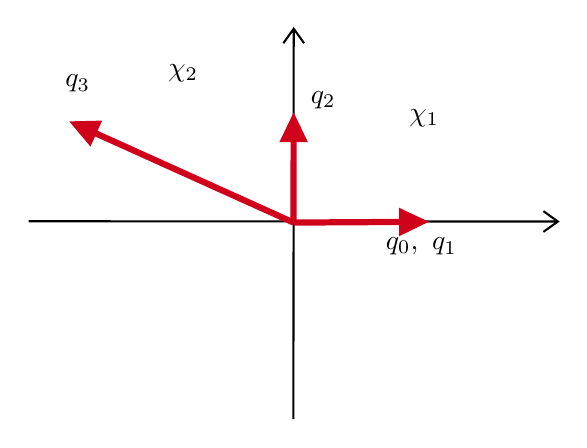
\begin{tikzpicture}[x=0.75pt,y=0.75pt,yscale=-1,xscale=1]
	%uncomment if require: \path (0,252); %set diagram left start at 0, and has height of 252
	
	%Shape: Axis 2D [id:dp521058933232561] 
	\draw [line width=0.75]  (220.97,123.04) -- (475.93,123.18)(348.65,30.28) -- (348.49,218.43) (468.93,118.17) -- (475.93,123.18) -- (468.92,128.17) (343.65,37.28) -- (348.65,30.28) -- (353.65,37.28)  ;
	%Straight Lines [id:da16836362624543133] 
	\draw [color={rgb, 255:red, 208; green, 2; blue, 27 }  ,draw opacity=1 ][line width=2.25]    (348.57,123.68) -- (348.61,75.61) ;
	\draw [shift={(348.62,70.61)}, rotate = 90.05] [fill={rgb, 255:red, 208; green, 2; blue, 27 }  ,fill opacity=1 ][line width=0.08]  [draw opacity=0] (14.29,-6.86) -- (0,0) -- (14.29,6.86) -- cycle    ;
	%Straight Lines [id:da8025190099366124] 
	\draw [color={rgb, 255:red, 208; green, 2; blue, 27 }  ,draw opacity=1 ][line width=2.25]    (348.57,123.68) -- (408.73,123.33) ;
	\draw [shift={(413.73,123.3)}, rotate = 179.67] [fill={rgb, 255:red, 208; green, 2; blue, 27 }  ,fill opacity=1 ][line width=0.08]  [draw opacity=0] (14.29,-6.86) -- (0,0) -- (14.29,6.86) -- cycle    ;
	%Straight Lines [id:da840019010653217] 
	\draw [color={rgb, 255:red, 208; green, 2; blue, 27 }  ,draw opacity=1 ][line width=2.25]    (348.57,123.68) -- (245.07,76.99) ;
	\draw [shift={(240.51,74.93)}, rotate = 24.28] [fill={rgb, 255:red, 208; green, 2; blue, 27 }  ,fill opacity=1 ][line width=0.08]  [draw opacity=0] (14.29,-6.86) -- (0,0) -- (14.29,6.86) -- cycle    ;
	
	% Text Node
	\draw (391.74,129.8) node [anchor=north west][inner sep=0.75pt]  [rotate=-0.04] [align=left] {$\displaystyle q_{0} ,\ q_{1}$};
	% Text Node
	\draw (355.61,59.24) node [anchor=north west][inner sep=0.75pt]  [rotate=-0.04] [align=left] {$\displaystyle q_{2}$};
	% Text Node
	\draw (237.33,51.28) node [anchor=north west][inner sep=0.75pt]  [rotate=-0.04] [align=left] {$\displaystyle q_{3}$};
	% Text Node
	\draw (403.06,67.91) node [anchor=north west][inner sep=0.75pt]  [rotate=-0.04] [align=left] {$\displaystyle \centerdot \chi _{1}$};
	% Text Node
	\draw (286.97,46.31) node [anchor=north west][inner sep=0.75pt]  [rotate=-0.04] [align=left] {$\displaystyle \centerdot \chi _{2}$};
	
\end{tikzpicture}
	
\end{centering}

Note that $\det V=(0,2)^T$
The characters define GIT quotients: 
\begin{itemize}
	\item  $X_{1}= \mathbb{C}^{4}//_{\chi_{1}}T^{2}= \mathbb{P}(\mathcal{O}_{\mathbb{P}^{1}}\oplus \mathcal{O}_{\mathbb{P}^{1}}(2)) = \mathbb{F}_2$
	\item  $X_{2}= \mathbb{C}^{4}//_{\chi_{2}}T^{2}= \mathbb{P}(1,1,2)$
\end{itemize}

Note that $\mathbb{F}_2$ is the minimal resolution of $\mathbb{P}(1,1,2)$, related by a blow up at its singular point.
\end{example}

Wall crossings can give us other standard birational transformations.

\begin{example}{Atiyah Flop}{Atiyah Flop}
Consider the action of $\mathbb{C}^{*}$ on $\mathbb{C}^3$ with weights $(1,1,-1)$. 
There are two quotients: $X_+$ corresponding to the chamber with the weights $(1,1)$, i.e. take the unstable locus to be $x=y= 0$, or $X_-$ corresponding to the chamber with $-1$, i.e. take unstable locus $z = 0$. With these stability conditions we have $$
X_{+}= \mathcal{O}(-1)_{\mathbb{P}^{1}} \qquad X_{-}= \mathbb{C}^2, $$ where the wall crossing from the $X_-$ to $X_+$ give the blow up at a point. 

Now suppose $\mathbb{C}^*$ now acts on $V = \mathbb{C}^4$  with coordinates $x_{1}, x_{2}, y_{1},y_{2}$, and weight matrix $Q = \begin{pmatrix}1&1&-1&-1\end{pmatrix}$. 
Defines two chambers in the secondary fan: $\chi_{+}>0$ and $\chi_{-}<0$, so we get unstable locus $x_{1}= x_{2}= 0$ and $y_{1}= y_{2}=0$. Hence $$
X_{+}\simeq \mathcal{O}(-1)_{\mathbb{P}^{1}}^{\oplus_{2}}\simeq X_-
$$This is an example of the Atiyah flop, related by a blow up and its flopping contraction. 
\end{example}

We say a variety is a minimal model if has nef canonical divisor. In the GIT picture, we say a GIT quotient is minimal if $-\det V$ lies in the closure of the chamber corresponding to the variety. 

\subsubsection{Wall Crossing Formula}

cf.~\cite{Kite_2022,ballard_mori_2013} Let $V$ be a vector space of dimension $n$, and let $T$ be an algebraic torus.

Let $V$ be a vector space of dimension $n$, and let $T$ be an algebraic torus. Denote $\det V = \sum_i q_i$, where $q_i$ is the $i^\mathrm{th}$ column of the weight matrix $Q$. 

\begin{definition}{1-Parameter Subgroup}{1-PS}
    Given a reductive, linear algebraic group $G$, we call a one parameter subgroup of $G$ (the image of) an injective homomorphism $\lambda : \mathbb{G}_{m}\to G$. If $G$ acts on a space $V$, this induces an action of $\mathbb{G}_m$ on $V$ defined by $\lambda$, of which we denote the fixed locus $V^\lambda$. 
\end{definition}

Consider a toric GIT problem defined by the action of a group $T$ on a vector space $V$. Let $C_+$ and $C_-$ be adjacent chambers of the secondary fan in $\mathbb{L}^{\vee}_\mathbb{R}$ separated by a wall $W$. Assume that $\det V$ is on the $C_{+}$ side of the adjoining wall $W$. The wall $W$ corresponds to an orthogonal (primitive) one-parameter subgroup $\lambda_{W}\in \mathbb{L}$.

We can define a value $\mu = (\det V)(\lambda_W)$. Let $\lambda_W$ be such that $\mu \geq 0$, so is pointing to the $C_-$ side of the wall. $\mu$ is a combinatorial value which will (roughly) tell us which chamber admits the `bigger' GIT quotients. 

Let $X_+$ (resp. $X_-$) be the GIT quotient $V // _{\theta_{+}}T$ (resp. $V // _{\theta_{-}}T$ ) corresponding to the chosen generic stability condition $\theta_{+}\in C_+$ (resp. $\theta_-$).  Recall from the previous section that GIT quotients are invariant across stability conditions in the interior of a given chamber. 

We can define a somewhat `smaller' GIT problem associated to a subset $S \subset \{ 1,\dots,n \}$, or more specifically a subset $Q_S$ of the weights corresponding to the set $S$, which in our case are the $s_i$ columns of the weight matrix for $s_{i}\in S$. These weights generate a sublattice $L_{S}^\vee\subset L_\mathbb{R}^\vee$, allowing us to define a GIT problem from the exact sequence $$M_{S}\to \mathbb{Z}^{S}\xrightarrow{Q_{S}}L_{S}^{\vee}$$

This GIT problem gives us a strictly lower dimensional variety $Z$, which is a GIT quotient of the fixed locus $V^{\lambda_{W}}$ by $T/\lambda_W$ (where here $T/ \lambda_W$ is the quotient by the image of $\mathbb{G}_m$ under $\lambda$). Here, our subset $Q_S$  is the collection of weights which are orthogonal to $\lambda_W$, that is, the weights which lie in the space spanned by $W$. We can see that lattice $\mathbb{L}_S^\vee$ is exactly the character lattice for the action of $T/\lambda_W$, since the the weights span the space orthogonal to $\lambda_W$. Moreover, the subspace of $V$ fixed by $\lambda_W$ corresponds to the lattice $\mathbb{Z}^S$ in the exact sequence. We choose a character $\theta_W$ in the interior of the wall $W$, to form the quotient $$Z = V^{\lambda_{W}} / /_{\theta_{W}} \left( T/ \lambda_{W}\right) . $$


\begin{definition}{Wall data}{}
	Given a wall $W$ in the secondary fan, define the Wall Datum as the tuple $(Z, \mu)$, where $\mu = (\det V)(\lambda_W)$ and $Z = V^{\lambda_{W}} / /_{\theta_{W}} \left( T/ \lambda_{W}\right)$ as described above. 
\end{definition}

Hence we get the theorem due to~\cite{halpernleistner2014derived} and~\cite{ballard2014variation}.

\begin{theorem}{Wall Crossing Formula}{wall crossing formula}
Consider GIT quotients $X_{+},X_{-}$  related by a wall crossing across W  with wall datum $(Z, \mu)$ as described above. 

If $\mu > 0$, we have a semi-orthogonal decomposition given by $$\mathcal{D}(X_{+}) = \left< \mathcal{D}(X_{-}),\mathcal{D}(Z) , \dots, \mathcal{D}(Z)  \right>$$ with $\mu$ copies of $\mathcal{D}(Z)$ appearing.

If $\mu = 0$, the wall crossing induces a flop, and we have an equivalence of categories $$\mathcal{D}(X_{+})\simeq \mathcal{D}(X_-).$$
\end{theorem}

This theorem was proved in~\cite{ballard2014variation} in much greater generality than used here, where such a decomposition holds for a smooth quasi-projective variety acted upon by a linear algebraic group, and a wall-crossing between two G-equivariant line bundles. However, to state the theorem in full generality requires more technical machinery than is necessary for the toric case for the purposes of our examples below. 

\begin{example}{}{}
    Recall Beilinson's exceptional collection~\cite{Beilinson1978} which forms a SOD of $\mathcal{D}(\mathbb{P}^n)$. Since $\mathbb{P}^n$ is a toric variety, we can realise it as the GIT quotient with respect to the usual action of $\mathbb{C}^*$ on $V = \mathbb{C}^{n+1}$. So the weights are $\begin{pmatrix}1 & 1 &\dots &1\end{pmatrix}$, with $\det V = n+1$. The wall crossing to $X_{-}=\emptyset$, retrieves the decomposition $\left< pt, \dots,pt \right>$ with $n+1$ copies of the derived category of a point, corresponding to the exceptional collection of line bundles on $\mathbb{P}^n$. 
\end{example}

\begin{example}{}{}
	Recall the wall crossing of example~\ref*{ex:Atiyah Flop}, where the action of $\mathbb{C}^{*}$ on $\mathbb{C}^3$ with weights $(1,1,-1)$ gives $$X_{+}= \mathcal{O}(-1)_{\mathbb{P}^{1}} \qquad X_{-}= \mathbb{C}^2, $$ The wall crossing formula gives us the decomposition $$\mathcal{D}(\mathcal{O}(-1)_{\mathbb{P}^{1}})= \left< \mathbb{C}^{2}, pt \right> $$ which recovers Orlov's blow-up formula from theorem~\ref*{thm:blowupformula}.
\end{example}

\begin{example}{}{}
    Now consider the action of $\mathbb{C}^{*}$ on $\mathbb{C}^3$ with weights $(1,1,-2)$ corresponding to coordinates $x_{1},x_{2},y_1,y_2$ .  Since $\det V = 0$, any wall crossing will give us a flop. Indeed, we have stability conditions, giving quotients $$X_{+}= \mathcal{O}_{\mathbb{P}^{1}}(-2) \qquad X_{-}= [\mathbb{C}^{2}/ \mathbb{Z}_2]  $$where $[\mathbb{C}^2/\mathbb{Z}_2]$ is the orbifold with the action of $\mathbb{Z}_2$. Then we get a derived equivalence $$\mathcal{D}(\mathcal{O}_{\mathbb{P}^{1}}(-2))\simeq \mathcal{D}([\mathbb{C}^{2}/\mathbb{Z}_{2}])$$
\end{example}


\subsubsection{Homological Mori Program}

The above theorem immediately yields a method for calculating a semi-orthogonal decomposition which is `maximally refined', in that none of its components can be factored further through wall-crossings. This follows a similar algorithm to the toric Mori program. Indeed, in such a GIT problem, a sequence of adjacent wall crossings come from sequences of birational operations, specifically directed flips, flops and divisorial contractions. This sequence can be seen by considering a path $\gamma : [0,1] \to \mathbb{L}^\vee$ in the cocharacter lattice, such that $\gamma(0)$ is in the ample cone of the secondary fan,$\gamma$ does not intersect a codimension 2 cone in $\mathbb{L}^\vee$, and $\gamma(1)$ is outside the support of the fan. Such a path $\gamma$ is called a run of the toric Mori program.

Starting with some fixed stability condition $\theta _1$ and its corresponding variety $X_1$, a wall crossing across the wall $W$ (away from $\det V$) gives the decomposition into $X_2$, the variety defined by the wall crossing, and $\mu$ copies of the variety $Z_W$, the variety defined by the wall datum for $W$. We can perform repeated wall crossings to decompose $X_2$ until a minimal model $X_{min}$ is reached. We will then be left with a factor of $X_{min}$ , and factors corresponding to the GIT problems $V^{\lambda_{W}} / / \lambda_{W}$ for each wall $W$ crossed, and can hence repeat the process of decomposition on each of the remaining non-minimal factors.

\begin{example}{Running the toric Mori program \cite{Kite_2022}}{}
	Let $(\mathbb{C}^*)^2$ act on $\mathbb{C}^6$ with weights $$Q = \begin{pmatrix}
		1&1&-1&0&0&0\\ 0&0&1&1&1&-1
	\end{pmatrix}$$
	Which gives secondary fan below
	\tikzset{every picture/.style={line width=0.75pt}} %set default line width to 0.75pt        

\begin{centering}	

	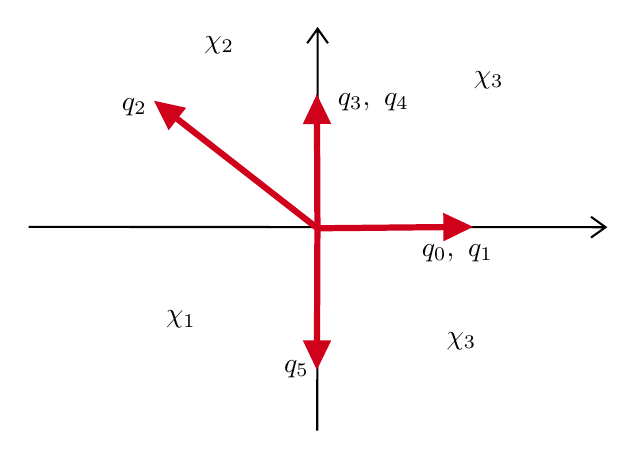
\begin{tikzpicture}[x=0.75pt,y=0.75pt,yscale=-1,xscale=1]
	%uncomment if require: \path (0,252); %set diagram left start at 0, and has height of 252
	
	%Shape: Axis 2D [id:dp521058933232561] 
	\draw [line width=0.75]  (211.98,127.56) -- (489.91,127.71)(351.16,32.07) -- (350.99,225.76) (482.91,122.7) -- (489.91,127.71) -- (482.9,132.7) (346.16,39.07) -- (351.16,32.07) -- (356.16,39.08)  ;
	%Straight Lines [id:da16836362624543133] 
	\draw [color={rgb, 255:red, 208; green, 2; blue, 27 }  ,draw opacity=1 ][line width=2.25]    (351.08,128.22) -- (350.84,68.69) ;
	\draw [shift={(350.82,63.69)}, rotate = 89.77] [fill={rgb, 255:red, 208; green, 2; blue, 27 }  ,fill opacity=1 ][line width=0.08]  [draw opacity=0] (14.29,-6.86) -- (0,0) -- (14.29,6.86) -- cycle    ;
	%Straight Lines [id:da8025190099366124] 
	\draw [color={rgb, 255:red, 208; green, 2; blue, 27 }  ,draw opacity=1 ][line width=2.25]    (351.08,128.22) -- (421.04,127.57) ;
	\draw [shift={(426.04,127.52)}, rotate = 179.47] [fill={rgb, 255:red, 208; green, 2; blue, 27 }  ,fill opacity=1 ][line width=0.08]  [draw opacity=0] (14.29,-6.86) -- (0,0) -- (14.29,6.86) -- cycle    ;
	%Straight Lines [id:da840019010653217] 
	\draw [color={rgb, 255:red, 208; green, 2; blue, 27 }  ,draw opacity=1 ][line width=2.25]    (351.08,128.22) -- (276.27,69.86) ;
	\draw [shift={(272.33,66.78)}, rotate = 37.96] [fill={rgb, 255:red, 208; green, 2; blue, 27 }  ,fill opacity=1 ][line width=0.08]  [draw opacity=0] (14.29,-6.86) -- (0,0) -- (14.29,6.86) -- cycle    ;
	%Straight Lines [id:da3402485134499953] 
	\draw [color={rgb, 255:red, 208; green, 2; blue, 27 }  ,draw opacity=1 ][line width=2.25]    (351.08,127.63) -- (350.84,191.49) ;
	\draw [shift={(350.82,196.49)}, rotate = 270.22] [fill={rgb, 255:red, 208; green, 2; blue, 27 }  ,fill opacity=1 ][line width=0.08]  [draw opacity=0] (14.29,-6.86) -- (0,0) -- (14.29,6.86) -- cycle    ;
	
	% Text Node
	\draw (400.12,134.79) node [anchor=north west][inner sep=0.75pt]  [rotate=-0.04] [align=left] {$\displaystyle q_{0} ,\ q_{1}$};
	% Text Node
	\draw (359.64,62.15) node [anchor=north west][inner sep=0.75pt]  [rotate=-0.04] [align=left] {$\displaystyle q_{3} ,\ q_{4}$};
	% Text Node
	\draw (255.65,64.24) node [anchor=north west][inner sep=0.75pt]  [rotate=-0.04] [align=left] {$\displaystyle q_{2}$};
	% Text Node
	\draw (276.88,166.81) node [anchor=north west][inner sep=0.75pt]  [rotate=-0.04] [align=left] {$\displaystyle \centerdot \chi _{1}$};
	% Text Node
	\draw (295.31,34.42) node [anchor=north west][inner sep=0.75pt]  [rotate=-0.04] [align=left] {$\displaystyle \centerdot \chi _{2}$};
	% Text Node
	\draw (333.78,190.58) node [anchor=north west][inner sep=0.75pt]   [align=left] {$\displaystyle q_{5}$};
	% Text Node
	\draw (425.14,51.51) node [anchor=north west][inner sep=0.75pt]  [rotate=-0.04] [align=left] {$\displaystyle \centerdot \chi _{3}$};
	% Text Node
	\draw (412.05,177.11) node [anchor=north west][inner sep=0.75pt]  [rotate=-0.04] [align=left] {$\displaystyle \centerdot \chi _{3}$};
	\end{tikzpicture}
	
\end{centering}

Since the anticanonical is $\begin{pmatrix}
	1\\2
\end{pmatrix}$, we will start the run of the toric Mori program in the chamber containing $\chi_3$, along a straight-line path intersecting the walls $\left<q_3,q_4\right>_+$ and $\left<q_2\right>_+$. 

The irrelevant ideal is $Irr(\chi_3) = \left< x_3 x_0,x_4 x_0, x_3 x_1 , x_4 x_1 , x_2 x_0 , x_2 x_1 \right>$, so the GIT quotient is $X_{3}= \mathbb{C}^6 \setminus X^{ss} (\chi_3)/ (\mathbb{C}^*)^2 = \mathrm{Tot} (\mathcal{O}(-1)_P)$ for $P = \mathbb{P}(\mathcal{O}^{\oplus 2} \oplus \mathcal{O}(-1))_{\mathbb{P}^1}$. From here, we cross the wall $\left<  q_{3}, q_4\right>_+$. $Irr(\chi_{2})= \left<  x_{2}x_{3}, x_{2}x_{4}, x_{2}x_{1}, x_{2}x_{0}\right>$, so $X_{2}= \mathbb{C}^{2} \setminus X^{ss}(\chi_{2})/ (\mathbb{C}^{*})^{2}= \mathcal{O}(-1)_{\mathbb{P}^3}$.  The wall between them has 1-PS $\begin{pmatrix}1\\0\end{pmatrix}$, so $\mu = 1$. $\mathrm{Tot }(\mathcal{O}(-1)_P)$ is a blow up of $\mathrm{Tot}(\mathcal{O}(-1)_{\mathbb{P}^3})$ along $\mathcal{O}(-1)_{\mathbb{P}^1}$, so the blow up formula gives wall data  $(Z = \mathcal{O}(-1)_{\mathbb{P}^1},1)$, giving the decomposition $$
\mathcal{D}(X_{3})= \left< X_{2}, \mathcal{O}(-1)_{\mathbb{P}^1} \right> 
$$
Now let's cross the wall $\left< q_2 \right>_+$. This has 1-PS $\begin{pmatrix}1\\1\end{pmatrix}$, so $\mu= 3$. 
$Irr (\chi_{1})= \left< x_{2}x_{5} \right>$, so $X_{1}= (\mathbb{C}^{6}\setminus \{ x_{2}= 0 \}\cup \{ x_{5}= 0 \})/ (\mathbb{C}^{*})^{2}= \mathbb{C}^4$. We can see that $\mathcal{O}(-1)_{\mathbb{P}^3}$ is the blow up of $\mathbb{C}^4$ at a point, so  the wall data is $(\mathbb{C}^{2} , 3)$, giving $$
\mathcal{D}(X_{2})= \left< pt, pt, pt , \mathbb{C}^2 \right> 
$$
Recall from Example~\ref{ex:Atiyah Flop}, $\mathcal{O}(-1)_{\mathbb{P}^1}$ is a toric GIT quotient defined by the blow up of $\mathbb{C}^2$ at a point, so we have $$
\mathcal{D}(\mathcal{O}(-2)_{\mathbb{P}^{1}})= \left<  pt, \mathbb{C}^2 \right> 
$$hence we have the decomposition $$
\mathcal{D}(X_{3}) = \left<  pt , \mathbb{C}^{2}, pt , pt, pt, \mathbb{C}^2 \right> .
$$

\end{example}

We are interested in finding examples of nontrivial equivalences of derived categories induced by flops, which in the toric picture can be seen by considering the Calabi-Yau case.From this, it is clear that $\mu = 0$ for all walls $W$ in the secondary fan, so any wall crossing induces a flop on the GIT quotients. Moreover, this gives us a way to see the nontrivial autoequivalences which come from these wall crossings. In particular, we will see that these autoequivalences have a nice interpretation as twists around spherical functors. 

\subsection{Windows and Spherical functors}

First, we want to make some generalizations on the theory of spherical objects. Recall that a spherical object $\mathcal{E} \in \mathcal{D}(X)$ satisfies the property that $$\mathrm{Hom}(\mathcal{E}, \mathcal{E}[i])= \begin{cases}
\mathbb{C} & i=0,\mathrm{dim}X  \\
0 & \text{otherwise}
\end{cases}$$
and the spherical twist of an object $\mathcal{F}$ around $\mathcal{E}$ is an autoequivalence defined as the cone $$T_\mathcal{E} = C(\mathrm{Hom}(\mathcal{E},\mathcal{F})\otimes \mathcal{E}\xrightarrow{ev} \mathcal{F})$$
We define spherical functors analogously.

\begin{definition}{}{}
	A functorial exact triangle is a `triangle' of exact functors $F_{1}, F_{2}, F_{3} : \mathcal{C}\to \mathcal{D}$,    equipped with natural transformations $$
F_{1}(-)\to F_{2}(-)\to F_{3}(-)\to F_{1}(-)[1]
$$ such that for every object $\mathcal{F}\in \mathcal{C}$,   we get the exact triangle in $\mathcal{D}$ given by $$
F_{1}(\mathcal{F})\to F_{2}(\mathcal{F})\to F_{3}(\mathcal{F})\to F_{1}(\mathcal{F})[1]
$$
\end{definition}

Consider an adjoint pair of exact functors $L \dashv R$. Let $\eta : \mathrm{Id}_\mathcal{D}\to R\circ L$ be the unit and $\epsilon : L\circ R \to \mathrm{Id}_\mathcal{C}$ the counit. 

\begin{definition}{}{}
A functor between triangulated categories $F: \mathcal{A}\to \mathcal{B}$ is called spherical if it admits an adjunction $F^{*}\dashv F$ and  functorial exact triangles 
\begin{align*}
F^{*}F \xrightarrow{\epsilon} \mathrm{Id}_\mathcal{A}&\to T \to F^{*}F [1] \\
C\to \mathrm{Id}_\mathcal{B}&\xrightarrow{\eta} F F^{*}\to C[1]
\end{align*} such that $T$ and $C$ are equivalences. Then we call $T$ (resp. $C$) the spherical twist(resp. cotwist) along $F$. 
\end{definition}

Let $X_+$ and $X_-$ be two toric varieties related by a flop induced from a wall crossing in a Calabi-Yau GIT problem. In the formulation of the wall-crossing decomposition, we get a variety $Z$ from the wall $W$ which may appear in as a factor. $Z$ is the toric variety arising from the GIT problem induced by a character on the ray spanned by the wall. In ~\cite{halpernleistner2016autoequivalences}, they show that we have countably infinitely many equivalences $\psi_{i}: \mathcal{D}(X_{-})\xrightarrow{\sim} \mathcal{D}(X_{+})$  such that the autoequivalence $\psi_{i+1}^{-1}\circ \psi_i$ of $\mathcal{D}(X_{-})$ is a spherical twist around a spherical functor $$F : \mathcal{G}\to \mathcal{D}(X_{-})$$ for a category $\mathcal{G}$ (to be defined later).

We examine this twist in more detail for the case of the standard flop (cf.~\cite{donovan_window_2014}) before stating the more general theorem. 

Recall once more the action of $T = \mathbb{C}^*$ on $V = \mathbb{C}^4$  acting on coordinates $x_{1}, x_{2}, y_{1},y_{2}$ with weights $\begin{pmatrix}1&1&-1&-1\end{pmatrix}$ respectively. So $X_+$ and $X_-$ are both isomorphic to $\mathcal{O}(-1)_{\mathbb{P}^1}^{\oplus_{2}}$, related by a flop along the zero section $\mathbb{P}^1_{x_{1},x_{2}}$ or vice versa. Clearly their derived categories are equivalent. Since $X_+$ and $X_-$ are the quotients of $V$ minus an unstable locus ($x_{1}= x_{2}= 0$ or $y_{1}= y_{2}=0$)  by $T = C^{*}$, we can view them as sub-quotient stacks of the Artin quotient stack $\mathfrak{X}=[V/T]$, with derived category $\mathcal{D}(\mathfrak{X})$. We thus have the inclusions $$
i_{\pm}: X_{\pm}\to \mathcal{X}
$$
Note that $\mathcal{D}(\mathfrak{X})$ contains the line bundles $\mathcal{O}(i)$ (corresponding to characters of $\mathbb{C}^*$).  Hence we define subcategories of $\mathcal{D}(\mathfrak{X})$ by $$
 \mathcal{W}_{t}= \left< \mathcal{O}(t), \mathcal{O}(t+1) \right> 
$$ for any $t \in \mathbb{Z}$. We can restrict the pullback of the inclusions to get equivalences $$
i^{*_{\pm}}:\mathcal{W}_{t} \xrightarrow{\sim} \mathcal{D}(X_{\pm})
$$
This equivalence can be verified by considering that $X_\pm$ is a quasi-projective variety, so we can make use of Beilinson's theorem stating that $\mathcal{O}(t), \mathcal{O}(t+1)$ is a strong, full, exceptional collection on $\mathbb{P}^1$, so the direct summands of the bundle $\mathcal{O}(t)\oplus \mathcal{O}(t+1)$ generate  $\mathcal{D}(\mathcal{O}(-1)_{\mathbb{P}^{1}}^{\oplus {2}})$.  Hence we can define the equivalence and then autoequivalence $$
\psi_{t}:= i_{+}\circ i_{-}^{*}: \mathcal{D}(X_{-})\to \mathcal{D}(X_{+}) \qquad \Phi_{t}:= \psi_{t-1}^{-1}\psi_{t}: \mathcal{D}(X_{-})\to \mathcal{D}(X_{-})
$$
We call $\mathcal{W}_t$ a window subcategory, in that $\mathcal{D}(X_{-})$is passing through a smaller intermediate than the whole of $\mathcal{D}(\mathfrak{X})$. Moreover, the autoequivalence can be composed from passing through any two windows, i.e. $$
w_{l,t}:= \psi_{l}^{-1}\psi_t
$$
This is called the `window shift'. 

\begin{remark}{}{}
	The method from this examples can be generalized to the action of $\mathbb{C}^*$ on $\mathbb{C}^k$ so long as the GIT problem is still Calabi-Yau. Assuming the sum of the positive weights is $d$ (so the sum of the negative weights is $-d$), window shift autoequivalences can be constructed with the subcategory $$\mathcal{W}_{t}= \left< \mathcal{O}(t),\dots, \mathcal{O}(t+d-1) \right> $$
\end{remark}


Consider the effect of $\Phi_t$ on our generators $\mathcal{O}(t)$ and $\mathcal{O}(t+1)$. Clearly $\psi_t$ sends both line bundles to themselves on $X_{+}$. Next we apply $\psi_{t-1}^{-1}$, but first both line bundles need to be resolved in such a way that they are written in terms of $\mathcal{O}(t-1)$ and $\mathcal{O}(t)$. We already have this for $\mathcal{O}(t)$. For $\mathcal{O}(t+1)$, the pullback of the Euler sequence on the zero section $\mathbb{P}^1$ gives the Koszul resolution $$
 0\to \mathcal{O}(2)\xrightarrow{\begin{pmatrix}x_2\\-x_{1}\end{pmatrix}}\mathcal{O}(1)^{\oplus 2}\xrightarrow{\begin{pmatrix}x_{1}&x_2\end{pmatrix}} \mathcal{O}
$$so $\mathcal{O}(t+1)$ is quasi-isomorphic to the complex $\left[ \mathcal{O}(t)^{\oplus{2}}\to \mathcal{O}(t-1) \right]$, and we have image of each generator under $\Phi_t$ . 
\begin{align*}
\mathcal{O}(t) &\mapsto \mathcal{O}(t)\\
\mathcal{\mathcal{O}}(t+1)&\mapsto\left[ \mathcal{O}(t)^{\oplus 2}\to \mathcal{O}(t-1) \right][-1] .
\end{align*}

We can see that computing the image of an arbitrary object in $\mathcal{E} \in \mathcal{D}(X_-)$ under $\Phi_t$ requires us to resolve $\mathcal{E}$ in terms of the generators of the first window, then resolve $\psi_{t}(\mathcal{E})$ in terms of generators of the second. This becomes more difficult in the general case.  \cite{donovan_window_2014} shows the existence of an endofunctor on the ambient quotient stack $\mathfrak{T}: \mathcal{D}(\mathfrak{X})\to \mathcal{D}(\mathfrak{X})$ which identifies objects from one window with another, called the Transfer Functor. To see it in action, let's consider the case of $t = 1$.

Since both $X_-$ and $X_+$ have exceptional locus $\mathbb{P}^1$, which can both be contracted to a point giving us the following maps $$
\left\{ pt \right\} \xleftarrow{\pi} \mathbb{P}^{1}\xrightarrow{j} X_{-}
$$
This can be generalised to maps from the substack identified with the quotient of $\mathbb{C}^{2}_{y_{1}, y_{2}} \oplus \{ 0 \}$ by $\mathbb{C}^*$, giving the correspondence $$
\{ pt \}\xleftarrow{\Pi}[\mathbb{C}^{2}/\mathbb{C}^*] \xrightarrow{J} \mathfrak{X}
$$
The transfer functor is then defined as the twist around the functor $\mathfrak{R}:= \Pi_{*}J^{!}: \mathcal{D}(X_{-})\to \mathcal{D}(\{ pt \})$  with left adjoint $\mathfrak{L}:= J_{*}\Pi^{*}$, given by $$
\mathfrak{T}:= \mathrm{Cone}\left(\mathfrak{L}\circ \mathfrak{R} \to \mathrm{Id}_{\mathcal{D}(\mathfrak{X})} \right) 
$$
This functor restricts to an autoequivalence $T: \mathcal{D}(X_{-})\to \mathcal{D}(X_-)$ which is similarly the twist for the adjunction $L\dashv R= \pi_{*}j^{!} : \mathcal{D}(X_{-})\to \mathcal{D}(\left\{ pt \right\})$. That is, $T$ fits into a functorial exact triangle $$
L\circ R \xrightarrow{\epsilon} \mathrm{Id}_{\mathcal{D}(X_{-})} \to T\to L\circ R[1]
$$Where $T$ is the cone on the counit $\epsilon$. 


\begin{theorem}{\cite{donovan_window_2014}}{}
	 $T$ is the same as $\Phi_1$. 
\end{theorem}

\begin{proof}
	
The proof of this statement relies on $\mathfrak{T}$ satisfying three key conditions. 

First, $\mathfrak{T}$ must send $\mathcal{W}_1$ to $\mathcal{W}_{0}$. This follows from that fact that the relative canonical sheaf $\omega_J$ of $J$ is $\mathcal{O}(-2)$ with relative dimension $-2$, so we have 
\begin{align*}
\Pi_{*}J^{!}(\mathcal{O}(1)) &= \Pi_{*}\left(\omega_{J}\otimes  J^{*} \mathcal{O}(1)[-2] \right) \\
&= \Pi_{*}\left( \mathcal{O}(-2)\otimes  J^{*}\mathcal{O}(1)[-2] \right) \\
&= \Pi_{*}\mathcal{O}(-1)[-2] \\
&=0  
\end{align*}

Hence $\mathfrak{L} \circ \mathfrak{R} (\mathcal{O}(1))=0$, and the cone on $\epsilon$ is the identity, so $\mathfrak{T}(\mathcal{O}(1)) = \mathcal{O}(1)\in \mathcal{W_0}$.

For $\mathcal{O}(2)$, 
\begin{align*}
\Pi_{*}J^{!}(\mathcal{O}(2)) &= \Pi_{*}\left(\omega_{J}\otimes  J^{*} \mathcal{O}(2)[-2] \right) \\
&= \Pi_{*}\left( \mathcal{O}(-2)\otimes  J^{*}\mathcal{O}(2)[-2] \right) \\
&= \Pi_{*}\mathcal{O}[-2] \\
&= \mathcal{O}_{pt}[-2]
\end{align*}

Pulling back from the point and pushing forward onto $\mathfrak{X}$, we get the sheaf $\mathcal{O}_{\mathbb{C}^{2}}[-2]$. We want to take the cone on the natural transformation $$
\mathcal{O}_{\mathbb{C}^2}[-2]\xrightarrow{\epsilon} \mathcal{O}(2)
$$ The exact sequence $$
0 \to \mathcal{O}(2)\to \mathcal{O}(1) ^{\oplus 2} \to \mathcal{O} \to \mathcal{O}_{\mathbb{C}^{2}}\to 0
$$ shows us that $\mathcal{O}_{\mathbb{C}^2}[-2]$ is quasi-isomorphic to $\left[ \mathcal{O}(2)\to \mathcal{O}(1)^{\oplus{2}}\to \mathcal{O} \right][-2]$, to taking the cone over $\epsilon$ gives us $\left[ \mathcal{O}^{\oplus{2}}\to \mathcal{O} \right][-1] \in \mathcal{W}_0.$

Hence we have 
\begin{align*}
\mathcal{O}(1) &\mapsto \mathcal{O}(1) \\
\mathcal{O}(2) &\mapsto \left[ \mathcal{O}(1)^{\oplus_{2}}\to \mathcal{O} \right][-2] 
\end{align*}

Which gives us the diagram

\[\begin{tikzcd}
	{\mathcal{W}_1} && {\mathcal{W}_0} \\
	& {\mathcal{D}(X_+ )} \\
	{\mathcal{D}(X_- )} && {\mathcal{D}(X_- )}
	\arrow["{\mathfrak T}", from=1-1, to=1-3]
	\arrow["{i_+^*}"', from=1-1, to=2-2]
	\arrow["{i_- ^*}"', from=1-1, to=3-1]
	\arrow["{i_+^*}", from=1-3, to=2-2]
	\arrow["{i_- ^*}", from=1-3, to=3-3]
	\arrow["{\psi_1}", from=3-1, to=2-2]
	\arrow["T", from=3-1, to=3-3]
	\arrow["{\psi_0}"', from=3-3, to=2-2]
\end{tikzcd}\]

Secondly, the upper triangle commutes because $\mathfrak{T}$ must act trivially outside $\mathbb{C}^{2}_{y_{1},y_{2}}\oplus \{ 0 \}$, i.e. $$
i^{*}_{+}\mathfrak{T} = i^{*}_{+}
$$This is a given from the definition, since objects on $X_+$ are in the kernel of the composition $\mathfrak{L}\circ\mathfrak{R}$, so $\mathfrak{T}$ acts as the identity. 

Thirdly,  $\mathfrak{T}$ must restrict to $T$, i.e. the rectangle commutes. This is due to generators $\mathcal{O}$ and $\mathcal{O}(-1)$ not having higher cohomology, so the derived pushforwards $\pi_{*}$ and $\Pi_{*}$ at least give the same thing on $\mathcal{W}_1$ , so $i_{-}^{*}\circ \mathfrak{T} = T\circ i_{-}^{*}$. 

From these, we can conclude that the lower triangle commutes, so $T = \Phi_1$. 
\end{proof}

To relate this back to the usual reference of spherical twist we can look at the functorial exact triangle object-wise, to see that for each object $\mathcal{E}\in \mathcal{D}(X_-)$, $T_F$ is the cone $$
T_{F}(E) = \mathrm{Cone}\left( \mathrm{Hom}(\mathcal{O}_{\mathbb{P}^{1}},\mathcal{E}) \otimes  \mathcal{O}_{\mathbb{P}^{1}} \to \mathcal{E}\right) 
$$ 

\begin{remark}{}{}
	This is just one example of a much more general statement about window shifts, and flops in general.~\cite{donovan_window_2014} prove the theorem for Grassmannian flops, which includes the case of the standard flop we just saw. Indeed, for  vector spaces $V$ and $S$ of dimension $d$ and $r \leq d$ respectively, the associated quotient stack for the GIT problem is $$
	\left[ \mathrm{Hom} (S,V) \oplus \mathrm{Hom}(V,S)/\mathrm{GL}(S) \right] 
	$$where the standard flop is the case when $d = 2$, $r=1$.
	\end{remark}

Indeed, the presentation of flop autoequivalences as spherical twists is not limited to GIT quotoients, as proved for a certain simplicity of wall crossings in~\cite{halpernleistner2016autoequivalences}. Barbocovi~\cite{barbacovi_spherical_2021} proves this fact for any flop which induces a derived equivalence, as summarised below.

Let $X_{-}\xleftarrow{p} \hat{X} \xrightarrow{q} X+$ be a flop. Moreover, assume that $p_{*}\mathcal{O}_{\hat{X}}= O_{X_-}$, $q_{*}\mathcal{O}_{\hat{X}}= O_{X_+}$,  and that there are derived equivalences$$
q_{*}p^{*}: \mathcal{D}(X_{-})\to \mathcal{D}(X_{+}), \qquad p_{*}q^{*}: \mathcal{D}(X_{+})\to \mathcal{D}(X_{-})
$$

Note that $p^*$ (resp. $q^{*}$) are left adjoints to $p_*$ (resp. $q_{*}$ ), and the properness and finite Tor dimension gives a right adjoint $p^{\times}: \mathcal{D}(X_{-})\to \mathcal{D}(\hat{X})$ and $q^{\times}: \mathcal{D}(X_{+})\to \mathcal{D}(\hat{X})$. Moreover, these left and right adjoints $p_{*}, p^{*} ,p^{\times}, q_{*}, q^{*},q^{\times}$ are all fully faithful, preserving boundedness and coherence.  

Define $\mathcal{K} = \mathrm{ker}(p_{*}) \cap \mathrm{ker}(q_{*})$ , and $\mathcal{ K}^{b}= \mathcal{K} \cap \mathcal{D}(\hat{X}) \subset \mathcal{D}(\hat{X})$. $\mathcal{K}^b$  is a thick full triangulated subcategory of $\mathcal{D}(\hat{X})$, hence we can take the quotient $Q: \mathcal{D}(\hat{X})\to \mathcal{D}(\hat{X})/\mathcal{K}^b$ , which gives us  induced maps
$$\bar{p}_{*} = \mathcal{D}(\bar{ X})/ \mathcal{K}^{b}\to \mathcal{D}(X_{-})$$

\begin{theorem}{Barbacovi}{}
There is a  four-periodic SOD of $\mathcal{D}(\hat{X})/\mathcal{K}^b$ given by $$
\left< \mathrm{ker}\,\bar{p}_{*},\mathcal{D}(X_{-}) \right> =  \left< \mathcal{D}(X_{+}), \mathrm{ker}\,\bar{q}_{*} \right> = \left< \mathrm{ker}\,\bar{q}_{*} , \mathcal{D}(X_{+})\right> = \left< \mathcal{D}(X_{-}), \mathrm{ker}\,\bar{p}_{*} \right>  
$$ which induces spherical functors $\Psi_{+}: \mathrm{ker} \bar{p}_{*}\xrightarrow{\bar{q}_{*}}\mathcal{D}(X_+)$ and $\Psi_{+}: \mathrm{ker} \bar{q}_{*}\xrightarrow{\bar{p}_{*}}\mathcal{D}(X_-)$ such that the `flop-flop' autoequivalences $FF _{+}:= q_{*}p^{*}p_{*}q^{*}$ and $F F_{-}: = p_{*}q^{*}q_{*}p^*$ are the spherical twists around each functor respectively.
\end{theorem}



\section{K3 surfaces and the cubic fourfold}

